\documentclass[11pt]{article}
\usepackage[T1]{fontenc}
\usepackage[utf8]{inputenc}
\usepackage{lmodern}
\usepackage[margin=1.05in]{geometry}
\usepackage{amsmath,amssymb,amsthm,mathtools}
\usepackage{microtype}
\usepackage{enumitem}
\usepackage{tikz}
\usetikzlibrary{arrows.meta,positioning,calc,patterns}
\usepackage{hyperref}
\hypersetup{colorlinks=true,linkcolor=black,citecolor=black,urlcolor=blue,
 pdftitle={Every complex K3 surface is Oka},pdfauthor={OpenAI}}
\newtheorem{theorem}{Theorem}[section]
\newtheorem{proposition}[theorem]{Proposition}
\newtheorem{lemma}[theorem]{Lemma}
\newtheorem{corollary}[theorem]{Corollary}
\theoremstyle{definition}
\newtheorem{definition}[theorem]{Definition}
\newtheorem{remark}[theorem]{Remark}
\newtheorem{example}[theorem]{Example}
\newcommand{\C}{\mathbb C}
\newcommand{\R}{\mathbb R}
\newcommand{\Z}{\mathbb Z}
\newcommand{\Q}{\mathbb Q}
\newcommand{\PP}{\mathbb P}
\newcommand{\B}{\mathbb B}
\newcommand{\dd}{\,\mathrm d}
\DeclareMathOperator{\ImPart}{Im}
\DeclareMathOperator{\RePart}{Re}
\DeclareMathOperator{\NS}{NS}
\DeclareMathOperator{\SO}{SO}
\DeclareMathOperator{\SU}{SU}
\DeclareMathOperator{\Aut}{Aut}
\DeclareMathOperator{\Pic}{Pic}
\DeclareMathOperator{\Spec}{Spec}
\DeclareMathOperator{\id}{id}
\setlist{itemsep=3pt,topsep=5pt}
\numberwithin{equation}{section}
\setlength{\emergencystretch}{2em}
\title{Every complex K3 surface is Oka}
\author{OpenAI}
\date{September 23, 2026}
\begin{document}
\maketitle
\begin{abstract}
We prove that every complex K3 surface $X$ is Oka, resolving the K3 Oka
conjecture. Equivalently, for every $m\geq1$, every holomorphic map to $X$
from a neighborhood of a compact convex set in $\C^m$ can be approximated
uniformly on that set by entire maps $\C^m\to X$.
\end{abstract}
{\small\tableofcontents}

\section{Introduction}\label{sec:introduction}

A \emph{complex K3 surface} is a compact connected complex surface that
is simply connected and has trivial canonical bundle. Thus it carries
a nowhere-zero holomorphic two-form. Every complex K3 surface is
K\"ahler, but it need not be projective or contain any curve
\cite[Chapters~1 and~7]{Huybrechts}. This combination of a rigid
cohomological structure and potentially sparse algebraic geometry makes
K3 surfaces a natural setting in which to study holomorphic flexibility.

The \emph{convex approximation property} (CAP) for a complex manifold
asks that maps holomorphic near a compact convex subset of $\C^m$ can
be approximated there by maps defined on all of $\C^m$, for every
source dimension $m$. Forstneri\v c proved that CAP characterizes Oka
manifolds \cite{ForstnericCAP,Forstneric}. In its equivalent Stein-source
formulation, the Oka property includes deformation of continuous maps
to holomorphic maps, with approximation and holomorphic interpolation.
Our main result is the following precise approximation statement.

\begin{theorem}\label{thm:main}
Let $X$ be a complex K3 surface, with any smooth Hermitian distance
$d_X$. For every integer $m\geq1$, every nonempty compact convex set
$K\subset\C^m$, every open neighborhood $U$ of $K$, every holomorphic
map $f:U\to X$, and every $\epsilon>0$, there exists a holomorphic map
$F:\C^m\to X$ such that
\[
                  \sup_{z\in K}d_X(F(z),f(z))<\epsilon.
\]
\end{theorem}

Theorem~\ref{thm:main} answers the K3 question in
\cite[Section~8, Problem~C]{ForstnericLarussonSurvey} and proves the
positive conjecture formulated explicitly in
\cite[Introduction]{XieZhao}. Its scope includes nonprojective
surfaces and imposes no condition on the Picard rank or existence of
an elliptic fibration.

An \emph{entire curve} is a holomorphic map from $\C$, and it is an
\emph{immersion} if its derivative never
vanishes. The approximation and interpolation theory gives the
following concrete consequence, proved in Section~\ref{sec:dense-entire}.

\begin{corollary}\label{cor:dense}
Let $S$ be a complex K3 surface. For every $x\in S$
and every nonzero vector $v\in T_xS$, there is a holomorphic immersion
$f:\C\to S$ such that
\[
 f(0)=x,\qquad f'(0)=v,\qquad \overline{f(\C)}=S,
\]
where closure is taken in the ordinary complex topology. If $S$ is
projective, then $f(\C)$ is Zariski dense.
\end{corollary}

Here the tangent vector, not just its line, is prescribed. For projective
$S$, the density conclusion confirms the K3 case of Campana's
prediction of Zariski-dense entire curves on special projective
manifolds \cite{Campana}. Here specialness means the absence of a
meromorphic fibration whose positive-dimensional base, endowed with
the orbifold structure induced by the multiple fibers, is of general
type.
See \cite[Conjecture~1.3]{CCR} for the prediction and
\cite[Proposition~8.9]{CCR} for the specialness of projective varieties
with trivial canonical bundle. The ordinary density and prescribed
first jet are additional conclusions.

Section~\ref{sec:surface-consequences} derives the Oka property for
Enriques surfaces and hence for all minimal compact complex surfaces
of Kodaira dimension zero. It also obtains global dominating sprays
on projective K3 and Enriques surfaces. A separate class-VII
classification there combines earlier Oka results with the global
spherical shell theorem of the companion manuscript \cite{OpenAIGSS};
that theorem is not an input to the K3 argument.

\subsection{Earlier results and the remaining obstacles}

The use of holomorphic sprays and approximation to realize topological
flexibility is central to Gromov's Oka principle for elliptic bundles
\cite{GromovOka}. Forstneri\v c's convex approximation characterization
\cite[Theorem~0.1]{ForstnericCAP} makes CAP an effective criterion for
this flexibility, while his interpolation theorem
\cite[Corollary~1.3]{ForstnericInterpolation} links it to prescribed
holomorphic data on subvarieties. Our proof uses local chart sprays
and splitting arguments in this tradition, with the uniform estimates
needed for the strip and convex-face constructions made explicit.

Holomorphic flexibility on K3 surfaces has been studied through entire
curves, domination by affine space, and approximation. Buzzard and Lu
proved that elliptic and Kummer K3 surfaces are holomorphically
dominable by $\C^2$ \cite[Propositions~4.4--4.5]{BuzzardLu}.
Dominability means the existence of a map $\C^2\to X$ whose
differential is surjective somewhere. Forstneri\v c and L\'arusson
strengthened this for every Kummer surface to \emph{strong
dominability}: such a map can pass through each prescribed target
point with surjective differential
\cite[Corollary~3]{ForstnericLarussonSurfaces}. These properties
concern individual maps; CAP asks for approximation of every local
map in every source dimension.

For arbitrary complex K3 surfaces, Kamenova, Lu and Verbitsky proved
that the Kobayashi pseudodistance vanishes
\cite[Corollary~2.2]{KamenovaLuVerbitsky}; the period-dynamics argument
is corrected in \cite[Section~4]{VerbitskyErratum}. This removes an
intrinsic obstruction to holomorphic flexibility, but does not
provide approximation or interpolation.

Alarc\'on and Forstneri\v c introduced the Oka-1 property and established
it for Kummer surfaces and elliptic K3 surfaces
\cite[Proposition~8.4 and Corollary~8.6]{AlarconForstneric}.
Oka-1 concerns approximation and discrete jet interpolation from open
Riemann surfaces, within prescribed continuous homotopy classes. Its
full formulation is recalled below.
The source dimension distinction matters: the one-dimensional
property alone does not give Theorem~\ref{thm:main}.

For projective K3 geometry, Chen, Gounelas and Liedtke developed
existence results for curves of prescribed geometric genus
\cite{ChenGounelasLiedtke}. Chen and Gounelas then proved that every
projective K3 surface contains genus-one curves of unbounded
self-intersection whose smooth normalizations vary in moduli
\cite[Theorem~A]{ChenGounelas}. We use two of their families with
different ample degrees. Their complete genus-one fibers supply
holomorphic flows for all complex times, and the difference in degrees
forces their tangent directions to be generically independent.

More recently, Xie and Zhao proved that smooth $(2,2,2)$ hypersurfaces
in $(\PP^1)^3$ are Oka and established dense $G_\delta$ sets of Oka
K3 periods and corresponding local deformation parameters
\cite[Theorems~A, B, and~E]{XieZhao}. Their work combines geometric
constructions of flexibility with arithmetic dynamics of periods and
Torelli theory. We use the same period-theoretic framework, including
the corrected orbit alternatives of Verbitsky
\cite{VerbitskyErratum}, with different geometric constructions.
A dense collection of Oka surfaces does not by itself settle the
property for each surface: the transfer must address every possible
rational subspace of its period plane.

Two analytic obstacles arise even before that transfer. Local
approximation in one variable must retain arbitrary holomorphic
parameters and then imply approximation on arbitrary convex sets.
Moreover, the geometric constructions produce long chains of annuli;
errors at their joins must be corrected without exhausting a fixed
positive transverse width. We handle the first issue by a polynomial
change of source coordinates and gluing estimates measured on real
faces. We handle the second by exact symplectic sewing with bounds
independent of the chain lengths.

\subsection{The proof and its organization}

The analytic and geometric parts meet at a local operation, denoted
$L$. It enlarges a planar disc across an attached disc, for maps with
image in a sufficiently small target neighborhood, while retaining
any prescribed smaller polydisc of passive holomorphic parameters.
Section~\ref{sec:local} defines $L$ precisely and obtains it from two
strip maps, one defined on $\C\times\Delta$ and the other on
$\Delta\times\C$, with transverse complete directions. Aligning
their coordinate axes exactly makes the overlap error arbitrarily
small. A bounded additive splitting and a contraction correct it.
The same section propagates $L$ across the center of a small disc
whose boundary already lies in the locus where $L$ holds.

Sections~\ref{sec:gluing} and~\ref{sec:globalization} prove that $L$
at every point implies CAP in every dimension
(Theorem~\ref{ana:cap}). A polynomial automorphism concentrates the
part of an enlarged polydisc outside the original domain into one
long coordinate and bounded transverse coordinates. The planar
operation with passive parameters then gives approximation on
polydiscs. To pass to an arbitrary convex set, we remove the defining
real faces of a containing polytope one at a time. The necessary
gluing estimate uses H\"older accuracy on each real face, without
requiring a fixed complex thickness on which that accuracy holds.

Section~\ref{sec:projective} constructs the two complete directions
on projective K3 surfaces using the Chen--Gounelas families. Propagation
across their algebraic exceptional set gives $L$ everywhere. This
handles one case of the final period argument and also exhibits a
direct source of the required local geometry.

The nonprojective cases require strips on open regions of period
space. Section~\ref{sew:section} first establishes the uniform sewing
theorem. On an annulus, a closed holomorphic one-form can have a
nonzero period. Exactness of the symplectic transition removes this
obstruction: the transverse constant Fourier coefficient becomes
quadratic in the error. The other Fourier modes admit a splitting
whose bounds are independent of the number and lengths of the
annuli. A quadratic iteration then retains a positive transverse
radius along an infinite chain.

To describe the geometric transfer, fix the K3 lattice $\Lambda$,
the integral second-cohomology lattice with its intersection form.
A \emph{marking} identifies $H^2(X,\Z)$ with $\Lambda$. The real
and imaginary parts of a nonzero holomorphic two-form span an
oriented positive two-plane, the \emph{period} of the marked surface.
Its rational directions are the vectors in its intersection with
$\Lambda\otimes\Q$.

Section~\ref{deg:section} constructs a nonempty open region in the
full period domain on which every surface has $L$ everywhere. It
smooths a union of two quadrics and sews annuli along their common
elliptic curve. The chart estimates persist under unrestricted small
K3 deformations. Section~\ref{rat:section} constructs a second kind
of region: for each fixed positive integral vector $v$, a relatively
open set among the period planes containing $v$. Here an isotrivial
genus-one fibration supplies the central model. Conservation of
imaginary symplectic action keeps all recentered annuli away from
singular fibers. Two independent cycles supply distinct strip leaves
after deformation and hence the transverse directions needed for $L$.

Finally, Section~\ref{dyn:section} applies Ratner's orbit theorem and
Verbitsky's corrected rational-direction analysis. Periods with no
rational direction have orbits meeting the first open region. Periods
with exactly one rational direction have orbits, under its stabilizer,
meeting the corresponding second region. Rational period planes give
projective K3 surfaces, already treated above. Torelli theory
transfers $L$ along these orbits, and Theorem~\ref{ana:cap} finishes
the proof. Section~\ref{sec:dense-entire} derives interpolation,
Corollary~\ref{cor:dense}, and the further surface consequences.

\paragraph{Conventions and standard inputs.}
Maps on a compact set are always defined on a neighborhood of that set.
Approximation may lose any prescribed positive amount of an auxiliary
domain margin. A strip means $\C\times\Delta_b$, with no injectivity
requirement unless stated; local regularity is specified at each use.
The analytic background consists of Stein theory, scalar approximation
and the $L^2$ $\bar\partial$ theorem
\cite{Forstneric,Hormander,Siu}. We recall the needed K3 period,
Torelli, and nef-pencil results at their applications
\cite[Chapters~2, 6--8, and~11]{Huybrechts}. The arithmetic inputs
are likewise stated where used. The local approximation, sewing,
geometric constructions, and reductions between them are proved here.


\section{Local approximation from complete directions}\label{sec:local}

The immediate goal is an operation that enlarges one planar source
variable while retaining arbitrary passive holomorphic parameters.
Two transverse complete strip maps provide this operation; a second
construction propagates it across points not initially covered by
strips. These are the inputs to the convex approximation argument
of Section~\ref{sec:globalization}.

Write $\Delta_r=\{z\in\C:|z|<r\}$. A map on a compact set will
always mean a map holomorphic on an open neighborhood of that set.
A \emph{special pair} $D\subset D'$ consists of two closed topological
discs with piecewise smooth boundary, where $D'$ is obtained from $D$
by attaching another such disc along a proper boundary arc. All
approximation assertions use an arbitrary fixed Hermitian distance
on the target.

\begin{definition}\label{loc:property}
A complex surface $X$ has property $L$ at $x$ if there is an open
neighborhood $V$ of $x$ with the following property. For every special
pair $D\subset D'$, every pair of closed polydiscs
$P_0\Subset\operatorname{int}P\subset\C^q$, and every holomorphic map
$f$ from a neighborhood of $D\times P$ into $V$, the restriction
$f|_{D\times P_0}$ is a uniform limit of maps holomorphic near
$D'\times P_0$ with values in $X$.
The case $q=0$ is included. We call $V$ a \emph{witness neighborhood}.
\end{definition}

Witness neighborhoods can be shrunk, and the locus where $L$ holds
is consequently open.

\subsection{Planar splitting and two strip maps}

In the first strip the first coordinate is complete; in the second
strip the second coordinate is complete. Their agreement below is
along a germ of the first strip's complete central curve and a transverse
starting section of the second strip, not along both complete
central curves. This agreement will make the overlap error small
without restricting either complete direction. The conclusion is
also allowed at a displaced point on the second strip's central
curve, a feature needed later when two leaves meet tangentially.

\begin{samepage}
\begin{proposition}[Two complete directions]\label{loc:criterion}
Suppose there are holomorphic maps
\[
\sigma_1:\C\times\Delta_b\longrightarrow X,\qquad
\sigma_2:\Delta_b\times\C\longrightarrow X
\]
which are locally biholomorphic at $(0,0)$ and satisfy
$\sigma_1(z,0)=\sigma_2(z,0)$ for small $z$. If $\sigma_2$ is
locally biholomorphic at $(0,c)$, then $L$ holds at
$x=\sigma_2(0,c)$.

The same conclusion holds for a sequence of pairs whose long
coordinate domains are discs of radii tending to infinity, whose
bounded-coordinate radii are bounded below, and whose maps converge
near $(0,0)$ and, for the second map, near $(0,c)$ to the above
nondegenerate germs. Exact axis agreement is required for every pair.
In this version $x$ is the value of the limiting second germ at $(0,c)$.
\end{proposition}
\end{samepage}

To construct an extension, we will choose a polynomial map
$h=(h_1,h_2)$ on the source. On one planar piece only $h_2$ must
be small, so that the first strip can be used; on the complementary
pieces only $h_1$ must be small, so that the second strip can be
used. Both coordinates are small on their overlaps. The next lemma
arranges these pieces while keeping the original disc in one of
the second-strip pieces.

\begin{lemma}\label{loc:pieces}
Given a special pair $D\subset D'$ and an open neighborhood $N$ of
$D$, there are compact sets $A,B_0,B_1\subset\C$ and bounded open
sets $U_A,U_0,U_1$ such that
\[
\begin{gathered}
\overline{U_A}\subset\operatorname{int}A,\qquad
\overline{U_i}\subset\operatorname{int}B_i\quad(i=0,1),\\
D\subset U_0,\qquad D'\subset U_A\cup U_0\cup U_1,\\
A\cap D=\varnothing,\qquad B_0\cap B_1=\varnothing,\qquad B_0\subset N.
\end{gathered}
\]
The compact sets $D\cup A$ and $B_0\cup B_1$ are polynomially convex.
For $U_B=U_0\cup U_1$, the two closed fringes
$\overline{U_A\setminus U_B}$ and $\overline{U_B\setminus U_A}$
have positive distance.
\end{lemma}

\begin{proof}
An ambient homeomorphism of the plane takes the attached-disc pair
to $D=[-2,0]\times[-1,1]$ and $D'=[-2,3]\times[-1,1]$.
Indeed, compatible parametrizations of the attaching arc and the
remaining boundary arcs extend over both discs by
Jordan--Schoenflies; the resulting outer boundary parametrization
extends across the exterior.
In this model choose
\[
0<c<c'<a'<a<b<b'<d'<d<3,\qquad 0<\delta<\epsilon.
\]
Use the following horizontal intervals:
\[
\begin{array}{c|c|c}
&\text{compact piece}&\text{open piece}\\ \hline
B_0,\ U_0&[-2-\epsilon,a]&(-2-\delta,a')\\
A,\ U_A&[c,d]&(c',d')\\
B_1,\ U_1&[b,3+\epsilon]&(b',3+\delta).
\end{array}
\]
All compact rectangles have vertical interval
$[-1-\epsilon,1+\epsilon]$, and all open rectangles have interval
$(-1-\delta,1+\delta)$. Take $a,\epsilon$ small enough that $B_0$
is in the prescribed neighborhood. The closed fringes are disjoint
compact sets, as is seen from their horizontal intervals
$[a',b']$ and $[-2-\delta,c']\cup[d',3+\delta]$.
Pull the sets back by the homeomorphism. Compact containment and
positive separation persist. The compact unions in the statement
are unions of two disjoint filled Jordan discs, hence have connected
complement and are polynomially convex.
\end{proof}

Figure~\ref{fig:pieces} displays the complementary coordinate control
for $h=(h_1,h_2)$: the first coordinate is small on the two outer pieces,
and the second is small on the middle piece.
\begin{figure}[ht]
\centering
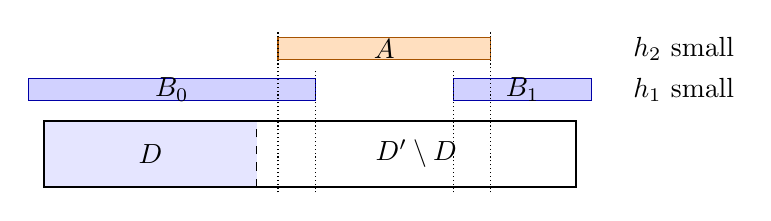
\begin{tikzpicture}[x=1.35cm,y=0.65cm]
 \fill[blue!10] (-2,-0.65) rectangle (0,0.65);
 \draw[thick] (-2,-0.65) rectangle (3,0.65);
 \draw[dashed] (0,-0.65)--(0,0.65);
 \node at (-1,0) {$D$};
 \node at (1.5,0) {$D'\setminus D$};
 \fill[blue!18] (-2.15,1.05) rectangle (0.55,1.48);
 \draw[blue!65!black] (-2.15,1.05) rectangle (0.55,1.48);
 \node at (-0.8,1.26) {$B_0$};
 \fill[blue!18] (1.85,1.05) rectangle (3.15,1.48);
 \draw[blue!65!black] (1.85,1.05) rectangle (3.15,1.48);
 \node at (2.5,1.26) {$B_1$};
 \fill[orange!25] (0.2,1.85) rectangle (2.2,2.28);
 \draw[orange!65!black] (0.2,1.85) rectangle (2.2,2.28);
 \node at (1.2,2.06) {$A$};
 \draw[densely dotted] (0.2,-0.75)--(0.2,2.4);
 \draw[densely dotted] (0.55,-0.75)--(0.55,1.65);
 \draw[densely dotted] (1.85,-0.75)--(1.85,1.65);
 \draw[densely dotted] (2.2,-0.75)--(2.2,2.4);
 \node[anchor=west] (first) at (3.45,1.26) {$h_1$ small};
 \node[anchor=west] (second) at (3.45,2.06) {$h_2$ small};
\end{tikzpicture}
\caption{Horizontal extents of the three compact pieces, shown in
separate rows. In the rectangular model, all three pieces share a vertical interval
slightly larger than that of $D'$. The two overlap bands control both
coordinates.}
\label{fig:pieces}
\end{figure}


The following is the additive Cousin splitting underlying holomorphic
spray gluing; compare \cite[Lemma~4.6]{ForstnericSplitting}.
We give its integral construction to retain bounds independent of the
number and radii of the passive parameters.

\begin{lemma}\label{loc:splitting}
Let $U_A,U_B\subset\C$ be bounded open sets with positively separated
closed fringes, and put $C=U_A\cap U_B$. For every open parameter
polydisc $P$ and every $k$, there are bounded linear operators
\[
\begin{aligned}
R_A&:H^\infty(C\times P,\C^k)\longrightarrow
H^\infty(U_A\times P,\C^k),\\
R_B&:H^\infty(C\times P,\C^k)\longrightarrow
H^\infty(U_B\times P,\C^k)
\end{aligned}
\]
satisfying $R_Au-R_Bu=u$. Their bounds depend only on the planar
sets and not on $P$ or its dimension.
\end{lemma}

\begin{proof}
Choose a smooth function $\chi$ on the plane, zero near
$\overline{U_A\setminus U_B}$ and one near
$\overline{U_B\setminus U_A}$, with bounded first derivative.
On $U_A$ extend $\chi u$ by zero off $C$; on $U_B$ extend
$(\chi-1)u$ similarly. Both extensions have planar
$\bar\partial$ derivative $u\bar\partial\chi$ on $C$ and zero
elsewhere in $\Omega=U_A\cup U_B$.
Extend this bounded coefficient by zero to $\C$ and set
\[
v(s,t)=\frac1\pi\int_C
 \frac{u(\zeta,t)\,\partial_{\bar\zeta}\chi(\zeta)}
      {s-\zeta}\,dA(\zeta).
\]
The distributional identity
$\partial_{\bar s}(1/(\pi s))=\delta_0$ gives the required
$\bar\partial$ equation. If $d$ is the diameter of $\Omega$, then
\[
\|v\|_{\Omega\times P}
\le 2d\|\bar\partial\chi\|_\infty\|u\|_{C\times P}.
\]
The kernel is locally integrable, so $v$ is continuous in $s$
and holomorphic in $t$. Thus
$R_Au=\chi u-v$ and $R_Bu=(\chi-1)u-v$ are holomorphic, have
the asserted bounds, and differ by $u$. No boundary continuity
of $u$ is needed.
\end{proof}

\begin{proof}[Proof of Proposition~\ref{loc:criterion}]
First consider complete strips. Choose $\rho>0$ so small that
$5\rho<b$, that
$\tau=\sigma_2^{-1}\circ\sigma_1$ is defined near
$\overline{\Delta}_{3\rho}^2$ using the inverse branch at the origin,
and that $D\tau$ is invertible there. Exact axis agreement gives
$\tau(z,0)=(z,0)$. The matrices $T_0(z)=D\tau(z,0)$ and their
inverses are bounded on $|z|\le2\rho$.
Choose a biholomorphic $\sigma_2$ chart $Q_c$ about $(0,c)$ whose
first coordinate has modulus less than $\rho/16$, and take a
relatively compact smaller image $V$ as the witness neighborhood.

Fix input data as in Definition~\ref{loc:property}. Choose an open
polydisc $P_*$ with
$P_0\Subset P_*\Subset\operatorname{int}P$.
In the chart $Q_c$ write $g=\sigma_2^{-1}\circ f=(g_1,g_2)$.
There is a planar neighborhood $N$ of $D$ where $g$ is defined for
parameters in a neighborhood of $\overline P_*$ and
$|g_1|<\rho/8$. No smallness of $g_2-c$ beyond membership in $Q_c$
is used in the overlap calculation.

Choose the pieces of Lemma~\ref{loc:pieces}. Products of polynomially
convex compact sets are polynomially convex. Scalar Oka--Weil
approximation therefore gives a polynomial $h_1$ in the planar and
parameter variables approximating $g_1$ on
$B_0\times\overline P_*$ and zero on $B_1\times\overline P_*$.
Its error $\epsilon_1$ can be arbitrarily small; in particular,
$|h_1|<\rho/2$ on their union. Independently, for every sufficiently
small $\eta>0$ there is a polynomial $h_2$ satisfying
\[
\|h_2-g_2\|_{D\times\overline P_*}<\eta,\qquad
\|h_2\|_{A\times\overline P_*}<\eta.
\]
Let $h=(h_1,h_2)$ and $C=U_A\cap U_B$. On $U_B\times P_*$,
$T=T_0(h_1)$ is holomorphic and boundedly invertible.
We seek corrections satisfying
\[
\tau(h+\alpha)=h+\beta,\qquad
\alpha=R_Au,\quad\beta=T R_Bu.
\]
By Lemma~\ref{loc:splitting}, this is the fixed-point equation
\[
u=\mathcal T(u):=
R_Au+T^{-1}\bigl(h-\tau(h+R_Au)\bigr)
\]
in $H^\infty(C\times P_*,\C^2)$.

On the overlap $|h_1|<\rho/2$ and $|h_2|<\eta$.
Bounded first and second derivatives of $\tau$, and its exact
axis identity, give a constant $M\ge1$ with
\[
\|T\|,\|T^{-1}\|\le M,\quad
\|\tau(h)-h\|\le M\eta,\quad
\|D\tau(h+\alpha)-T\|\le M(\eta+\|\alpha\|).
\]
These constants do not depend on the degrees or uncontrolled
coordinates of the polynomials. If $\kappa\ge1$ bounds both
splitting operators and $L_0=2M^2+1$, then on $\|u\|\le L_0\eta$,
\[
\|\mathcal T(0)\|\le M^2\eta,\qquad
\|D\mathcal T(u)\|\le
M^2\kappa(1+\kappa L_0)\eta.
\]
For small $\eta$ the last bound is at most $1/2$, the ball maps
strictly into itself, and all transition evaluations remain in
$\Delta_{3\rho}^2$. The contraction theorem gives
\[
\|\alpha\|\le\kappa L_0\eta,\qquad
\|\beta\|\le M\kappa L_0\eta.
\]

On $U_A\times P_*$ only the second coordinate of $h+\alpha$ has
to be small, and on $U_B\times P_*$ only the first coordinate
of $h+\beta$ has to be small. Consequently
$\sigma_1(h+\alpha)$ and $\sigma_2(h+\beta)$ are defined on
these full domains and agree on their overlap. On $D\times P_*$,
the second formula is evaluated close to $g$ in $Q_c$ and
approximates $f$ as $\epsilon_1,\eta\to0$. Since the union of the
planar domains contains $D'$ and $P_0\Subset P_*$, this proves $L$.

For the finite-length version choose $V$, $g$, and the two
polynomials using the limiting chart at $(0,c)$. Convergence on
slightly larger compact coordinate neighborhoods gives uniform
first and second derivative bounds, uniform inverse-chart domains,
and thus uniform constants in the contraction argument.
Exact axis agreement gives the same $O(\eta)$ initial error for
every pair. The polynomials are bounded on the fixed bounded
planar pieces and $\overline P_*$, so only a finite range of either
long coordinate is used. Choose a sufficiently late pair to contain
these ranges and make its chart near $(0,c)$ sufficiently close to
the limiting chart. The construction then approximates the original
data with the requested accuracy.
\end{proof}

\begin{remark}\label{loc:alignment}
Two strip maps locally biholomorphic at chosen meeting preimages,
with transverse central curves there, can be put in the form of
Proposition~\ref{loc:criterion}. Locally lift the
first central curve through the inverse of the second strip, writing
the lift as $(a(z),t(z))$, where its bounded coordinate is $a$.
Replace the second strip by
$\widetilde\sigma_2(z,w)=\sigma_2(a(z),t(z)+w)$.
Transversality says $a'(0)\ne0$, and time zero gives exact axis
agreement. If the original second central curve also passes through
$x$ and its strip is regular there, some finite $c$ gives a regular
chart $\widetilde\sigma_2(0,c)=x$.
For finite-length families whose central germs converge to transverse
germs through a common point, the implicit function theorem first
gives nearby intersection points and meeting preimages. Translate
the preimages to the origin and apply the same construction.
Convergence and transversality give a uniformly positive
bounded-coordinate radius; the translations and the function $t$
lose only a bounded amount of long-coordinate length. Thus this
construction also supplies the aligned families in the finite-length
part of the proposition.
\end{remark}

\subsection{Sprays, deformation, and planar gluing}

The strip criterion provides approximation when all input values lie
in one witness neighborhood. To apply it successively to a map whose
image meets several such neighborhoods, we need coordinates around
the graph of the map and a way to join close maps in those coordinates.
The next three lemmas supply exactly these tools. The use of sprays
and their gluing follows the framework of Gromov \cite{GromovOka}
and Forstneri\v c \cite{Forstneric}; here the sprays are constructed
only near the graph on a relatively compact Stein source.

\begin{lemma}[Local chart sprays]\label{loc:spray}
Let $f:S\to X$ be holomorphic on a Stein manifold, let
$K\Subset S$ be compact, and assume $f^*TX$ is holomorphically
trivial on $S$. After shrinking the source neighborhood there
is a holomorphic map $f^\sharp(z,v)$ for $z$ near $K$ and
$v\in\Delta_r^2$, with $f^\sharp(z,0)=f(z)$, such that
$v\mapsto f^\sharp(z,v)$ is injective with invertible differential.
The hypothesis on $f^*TX$ holds for a contractible Stein source
and for a planar domain times a polydisc.
\end{lemma}

\begin{proof}
The graph of $f$ is a closed Stein submanifold of $S\times X$ and
has a Stein neighborhood by the Stein neighborhood theorem
\cite{Siu}. On that neighborhood consider the vertical tangent
bundle for projection to $S$. A holomorphic frame along the graph
extends to holomorphic vertical vector fields by Cartan's
Theorem~B. Compose their small-time flows. The resulting map has
the prescribed value and a frame as its vertical differential
at $v=0$. Compactness and the holomorphic inverse function theorem
give a common radius on a neighborhood of $K$ and injectivity
in each parameter fiber.
For the last assertion, a planar domain has the homotopy type of
a one-dimensional CW complex, so every complex vector bundle on
its product with a polydisc is topologically trivial. The
Oka--Grauert principle makes it holomorphically trivial.
The same argument applies to a contractible Stein source
\cite{Forstneric}.
\end{proof}

\begin{lemma}[Deforming a map on a relatively compact Stein domain]
\label{loc:deformation}
Let $\pi:\mathcal X\to B$ be a holomorphic family, and let
$f:S\to\mathcal X_{b_0}$ be holomorphic from a Stein manifold
with image in the submersion locus of $\pi$. On every relatively
compact source domain there is a holomorphic family of maps
$f_b$ into $\mathcal X_b$ for $b$ near $b_0$, with $f_{b_0}=f$.
\end{lemma}

\begin{proof}
Work in local coordinates on $B$ at $b_0$. The graph of $f$ has
a Stein neighborhood in $S$ times the submersion locus. On this
neighborhood the surjection from tangent vectors vertical over $S$
to the pulled-back base tangent bundle admits holomorphic lifts of
the base coordinate vector fields: its kernel is coherent, and
Cartan's Theorem~B gives surjectivity on global sections. Flow the
lifts successively for the small coordinate displacements of $b$.
On a relatively compact source set a common time radius is
available. The flows are vertical over $S$, and their projections
to $B$ are the desired coordinate translations. Their composition
is the required family of maps.
\end{proof}

\begin{lemma}[Planar spray gluing]\label{loc:gluing}
Suppose two holomorphic sprays over bounded planar domains $U_A,U_B$ and
a parameter polydisc are uniformly close on their overlap, with
a positive margin in an auxiliary spray polydisc. Suppose the
first spray is a chart spray there with uniform inverse-chart
margins, and the closed planar fringes
are positively separated. If the closeness is sufficiently small,
their central maps can be glued after arbitrarily small
holomorphic corrections in the auxiliary variables. The glued
map is arbitrarily close to the first central map on any prescribed
compact subset of its domain on which that spray is fixed, or has
a uniform modulus of continuity in its auxiliary variables.
\end{lemma}

\begin{proof}
Write the sprays as $F_A$ and $F_B$. Compact chart margins give
the transition
$\gamma(s,t,v)=F_A(s,t,\cdot)^{-1}(F_B(s,t,v))
=v+E(s,t,v)$ on the overlap, with both
$\|E\|$ and $\|D_vE\|$ small on a smaller auxiliary polydisc.
The derivative estimate follows from the original closeness by
Cauchy estimates on the larger polydisc. Equality of the resulting
maps asks for $a=\gamma(b)$.
Use $a=R_Au$, $b=R_Bu$. Then
\[
u=E(s,t,R_Bu)
\]
is a contraction on a small ball in the overlap $H^\infty$ space.
Lemma~\ref{loc:splitting} supplies its uniform bounds and preserves
holomorphic dependence on the passive parameters. The resulting
corrections remain in the auxiliary polydisc and are as small
as the original mismatch. Uniform continuity on the prescribed
compact sets gives the asserted approximation.
\end{proof}

The domains in this lemma may be thin neighborhoods of compact
planar sets. In applications below the cutoff is chosen first on
a fixed overlap band. Its derivative bound, and the diameter bound
in Lemma~\ref{loc:splitting}, do not increase when the domains are
subsequently narrowed away from that band.

\subsection{One planar enlargement with passive parameters}

\begin{proposition}\label{loc:planar}
Let $K$ be a closed circular disc of radius $r$, or a closed
circular annulus with outer radius $r$, and let $f$ be holomorphic
near $K\times P$, where $P$ is a closed polydisc. Suppose that for
every $\zeta$ on the outer circle there is a coordinate witness
neighborhood $V_\zeta$ for $L$ containing $f(\{\zeta\}\times P)$.
For every $R>r$ and $P_0\Subset\operatorname{int}P$, one can
approximate $f$ uniformly on $K\times P_0$ by a map holomorphic
near the enlarged disc, respectively annulus with the same inner
radius and outer radius $R$, times $P_0$.
\end{proposition}

\begin{proof}
We give a finite construction with explicit approximation margins.
Choose a compact intermediate parameter polydisc strictly between
$P_0$ and $P$. Compactness gives a partition of the outer circle
into finitely many closed arcs, with endpoint margins, such that
all values over each slightly enlarged arc and the intermediate
parameter set lie in one coordinate witness neighborhood $V_j$.
At the common endpoint of consecutive arcs the compact set of
values lies in $V_j\cap V_{j+1}$ with a positive target margin.
Take a slightly larger outer radius than $R$ during the construction.

\emph{Attach radial spokes.}
At each endpoint choose a small filled polar rectangle crossing
the old outer circle, on which $f$ and a chart spray from
Lemma~\ref{loc:spray} have their values in both adjacent target
charts. The rectangles can be chosen mutually disjoint. Attach
to each rectangle a radial segment reaching the larger outer
radius. In one of its target charts, continue the coordinate
spray constantly along the segment from its attachment point on
the outer edge of the rectangle. This defines continuous
coordinate functions on the filled rectangle and attached segment,
holomorphic on its interior and holomorphic in the passive and
auxiliary parameters.

The planar compact set has connected complement. Mergelyan
approximation, with parameters, approximates these coordinate
functions by polynomials. Here the parameter assertion follows
directly by taking finite Taylor sums on a slightly larger
parameter polydisc and applying scalar Mergelyan to their
coefficients. Consequently the approximation can be made uniform
with an auxiliary-parameter margin, and Cauchy estimates preserve
the required spray derivatives. On the radial segment its values
remain close to the endpoint values for all parameters. A thin
neighborhood of each segment therefore also has its values in
both adjacent $V_j$'s.

Glue this extension to the old chart spray across a radial band
inside each original rectangle, using Lemma~\ref{loc:gluing}.
More explicitly, cut the union domain at a radius slightly larger
than $r$, still inside the old map domain. At the cut it consists
only of the disjoint rectangles. A radial cutoff with a fixed
transition width gives separated fringes and a bounded splitting
constant. The tubes around the longer portions of the spokes may
then be narrowed without changing that constant. Gluing errors
can be as small as desired. This produces a map near $K$ and all
spokes, close to $f$ on $K$, with all spoke values still in the
two adjacent target charts.

\emph{Fill the sectors.}
List the finitely many closed polar sectors between successive
spokes. At a given step let $K_{\rm old}$ be the union of the
original compact set, all spokes, and the sectors already filled.
The next sector $S$ meets $K_{\rm old}$ exactly on its bottom
arc and its two radial sides. Along these three sides all map
values, with a parameter margin, belong to the chosen $V_j$.
This is true initially by the spoke construction, and it remains
true after each sufficiently accurate gluing, because the sides
of every unfilled sector already belong to $K_{\rm old}$.

Choose a thin closed U-shaped band $D$ about these three sides,
inside the current map domain, and a slightly enlarged filled
sector $D'$ containing $S$ in its interior, so that $D\subset D'$
is a special pair. To see this elementary geometry, straighten
the sector to a rectangle: $D$ is a thick band around its bottom
and two side edges, and the missing central rectangle attaches
along the U-shaped portion of its boundary. The bands and
protrusions can be made as thin as needed.
All values near $D$ lie in $V_j$. Apply $L$ to the restriction
of a chart spray over the current map, regarding its small
auxiliary variables as additional passive parameters. After any
prescribed small parameter loss this gives a spray on $D'$,
arbitrarily close to the old spray on $D$.

We spell out the overlap used to glue. Fix an open band
$W\Subset\operatorname{int}D$ containing $K_{\rm old}\cap S$.
Using a slightly smaller band first, the compact remainders on
opposite sides are positively separated. A smooth cutoff can
therefore be zero near $K_{\rm old}\setminus W$ and one near
$S\setminus W$. On a sufficiently thin neighborhood of
$K_{\rm old}\cup S$, its sublevel and superlevel sets give two
open domains with separated fringes and overlap contained in $W$.
They may be chosen so that any point of $K_{\rm old}$ in the new
side also lies in the approximation band. The old spray is
defined on the first domain, the approximating spray on the
second, and they are close on their overlap with an auxiliary
margin. Lemma~\ref{loc:gluing} produces the required new map,
close to the old map on all of $K_{\rm old}$.

There are only finitely many spokes and sectors. Fix in advance
a finite nested sequence of parameter polydiscs between the
intermediate one and $P_0$. At each step choose errors smaller
than the remaining compact target-chart margins and allocate a
summable finite part of the requested final error. These choices
preserve every unfilled sector's joining sides. No chart condition
on the outer boundary of a newly filled sector is required.
At the end we have a map on a neighborhood of the desired
enlarged compact set times $P_0$, with the stated approximation.
\end{proof}

\begin{corollary}[Propagation across a small disc]\label{loc:disc}
Suppose a coordinate neighborhood contains a closed affine
complex-line disc centered at $x$, with its boundary in the open
locus where $L$ holds. Then $L$ holds at $x$.
In particular, if the complement of that locus is contained
locally in a proper analytic subset, $L$ holds everywhere.
\end{corollary}

\begin{proof}
Slightly tilt the line in two different directions through $x$.
Openness and compactness of the original boundary imply that the
two tilted discs still have boundary in the good locus, and their
tangent directions at $x$ are transverse. Thicken each disc in a
complementary coordinate by a sufficiently small fixed parameter
disc. At every boundary point the values for all parameters then
lie in one witness neighborhood; finitely many boundary patches
give one common positive transverse radius.

For each integer $n$, apply Proposition~\ref{loc:planar} once to
each thickened disc, enlarging its long coordinate to radius
$n$, retaining a fixed smaller transverse radius, and making its
error on the initial product less than $1/n$. The resulting
finite strips converge near their centers to the original
coordinate charts. Their limiting long directions are transverse.
Remark~\ref{loc:alignment} and the finite-length case of
Proposition~\ref{loc:criterion} imply $L$ at $x$.

If a proper analytic subset $E$ contains the exceptional points
in a coordinate neighborhood of $x$, choose a complex line
through $x$ not contained in $E$. Its intersection with $E$ is
discrete near $x$, so a sufficiently small circle on that line
avoids $E$. The first assertion applies.
\end{proof}

\begin{remark}
The proof also records a useful uniform version: finitely many
coordinate discs whose boundaries lie in fixed compact subsets of
the good locus retain the required boundary containment after
sufficiently small deformations of the coordinate charts.
All arguments in this section concern one planar variable with
passive parameters. No approximation theorem for arbitrary
multidimensional source compacta has been used.
\end{remark}

\section{Approximation on polydiscs}
\label{sec:gluing}

We now pass from the planar operation $L$ to approximation in every
source dimension. The first step is to enlarge a polydisc. A change
of source coordinates will put the part beyond the original map domain
into the form of one long planar variable with bounded passive
variables. Near the joining annulus, the passive variables describe
sets of arbitrarily small diameter, so that $L$ applies to their
images in a single witness neighborhood. We then join this extension
to the original map on a buffered open overlap.

Write
\[
 \overline\Delta_R^{\,m}=\{z\in\C^m:\max_j|z_j|\leq R\},
 \qquad \|z\|_\infty=\max_j|z_j|.
\]
All holomorphic maps on compact sets below are defined on open
neighborhoods of those sets.  Extra polydiscs always have positive
radii.  A zero-dimensional polydisc is allowed.

\begin{theorem}\label{ana:cap}
Let \(Y\) be a complex surface with a complete compatible distance.
If the local operation \(L\) holds at every point of \(Y\), then \(Y\)
has the convex approximation property in every source dimension.
\end{theorem}

This section proves the polydisc case. Section~\ref{sec:globalization}
will remove the remaining restriction on the shape of the convex set.

\subsection{Gluing on a buffered open overlap}

The source change need not preserve product overlaps, so the planar
splitting of Lemma~\ref{loc:splitting} must be replaced by a splitting
on a convex neighborhood in $\C^n$. Let $Q\subset\C^n$ be compact
and convex, and put $Q_r=\{z:\operatorname{dist}(z,Q)<r\}$ for $r>0$.
An auxiliary variable $v$ ranges over a ball $B_b\subset\C^N$;
the splitting operators below act only on $z$ and preserve
holomorphic dependence on $v$.

Suppose two open sets
$A,B$ cover a neighborhood of $\overline{Q_r}$ and have a fixed buffered
overlap: there is a smooth cutoff equal to zero near $A\setminus B$ and
one near $B\setminus A$, whose transition lies inside $A\cap B$ with a
positive collar. The collar is understood relative to the total domain;
after shrinking $Q_r$ its width has a positive lower bound depending
only on the fixed geometry. For a bounded holomorphic jump $u$,
the functions $\chi u$ and $(\chi-1)u$, extended by zero where their
respective multipliers vanish, have the same $\bar\partial$ derivative.
Fix $0<h<\min(r/2,1)$. The constants below depend only on the fixed
overlap geometry, a bounded range of $r$, and the dimensions, not on
the jump $u$ or its holomorphic auxiliary parameters.
Solve this common equation on an intermediate convex thickening,
using the weighted minimal $L^2$ solution with weight $|z|^2$
\cite[Theorem~2.2.1$'$]{HormanderLTwo}. The weight is bounded above
and below on the fixed bounded domains, so the solution has $L^2$
norm at most a fixed constant times that of the input form.
Cauchy estimates on the buffered transition region control any fixed
number of derivatives of that form by powers of $h^{-1}\|u\|_\infty$.
Interior elliptic estimates, applied to
$\Delta w=4\sum_j\partial\eta_j/\partial z_j$ when
$\bar\partial w=\sum_j\eta_j\,d\bar z_j$, give the corresponding
supremum bound for $w$ on the smaller thickening. Subtracting $w$
from the two cutoff functions gives bounded linear splittings on
$A\cap Q_{r-h}$ and $B\cap Q_{r-h}$, with bound
$Ch^{-p}\|u\|_\infty$ for some fixed integer $p$.
The minimal solution operator is linear and fixed on the base domain;
it therefore preserves holomorphic auxiliary parameters.

\begin{lemma}[Small nonlinear gluing on an open overlap]\label{glue:open}
In the preceding buffered open-overlap geometry, let two holomorphic
sprays into a complex manifold be related on their overlap by a fiber
coordinate change
\[
 \gamma(z,v)=v+c(z,v),\qquad v\in B_b.
\]
Suppose $\|c\|_\infty$ can be made arbitrarily small with $b>0$ fixed.
After any prescribed positive loss of base and fiber margins, the two
sprays admit fiber reparametrizations close to the identity which make
them agree. Evaluating at $v=0$ gives a glued holomorphic map. It is
arbitrarily close to the original map on each compactum where the
corresponding input spray is fixed, or has a uniform modulus of
continuity in the fiber variable. No such uniform target estimate is
asserted on a side whose spray varies without this control.
\end{lemma}

\begin{proof}
Use the additive splitting to find $a,b$ with $b-a=c$. Shrink the
base and fiber domains by $h$. The splitting bounds and Cauchy
estimates in $v$ imply, with a fixed integer $p$ enlarged as necessary,
\[
 \|a\|+\|b\|\le Ch^{-p}e,\qquad e=\|c\|,
\]
including their needed fiber derivatives on intermediate smaller balls.
For $Ch^{-p}e$ sufficiently small relative to these margins,
$\operatorname{id}+b$ has a fiber inverse on a smaller ball, uniformly
in the base. The new transition is
\[
 (\operatorname{id}+b)^{-1}\circ\gamma\circ(\operatorname{id}+a)
       =\operatorname{id}+d.
\]
The equation determining $d$ is
\[
 d= c(v+a)-c(v)-\{b(v+d)-b(v)\}.
\]
The first difference is quadratic in $e$, up to powers of $h^{-1}$.
The operation in braces is contractive on a small supremum-norm ball,
by the first fiber derivative bound. It follows that
\begin{equation}\label{eq:glue-quadratic}
             \|d\|\le Ch^{-p}e^2.
\end{equation}
These estimates involve a fixed finite number of derivatives. Thus one
common exponent $p$ works throughout the iteration; no derivatives of
increasing order are requested.

Choose losses $h_i=h_0 2^{-i}$ whose sum fits within the prescribed
margins, leaving intermediate buffers at each step. With
$A=Ch_0^{-p}$, Equation~\eqref{eq:glue-quadratic} reads
$e_{i+1}\le A2^{pi}e_i^2$. Put $E_i=A2^{p(i+1)}e_i$. Then
$E_{i+1}\le E_i^2$. Choosing $E_0<1/2$ gives doubly exponential decay.
In particular all sums $\sum_i h_i^{-q}e_i$ converge for every fixed
$q$, and are as small as desired with $e_0$.

The successive fiber reparametrizations are composed on the nested
domains. Their displacements fit within the reserved buffers and their
fiber derivatives have summable deviations from the identity. The
compositions therefore converge uniformly. Their limiting transitions
are the identity.
Composing the two original sprays with these limiting side maps gives
equal maps on the overlap.
The target approximation assertion follows from the stated continuity
control and the smallness of the limiting fiber corrections.
\end{proof}

\subsection{A change of coordinates with a thin parameter range}

Enlarging one coordinate of a polydisc directly leaves an entire
transverse polydisc over each boundary point; its image need not fit
one witness neighborhood for $L$. We instead deform the source by a
polynomial automorphism. It will be nearly the identity on the old
polydisc, while the rest of the enlarged source has coordinates
$(s,\xi)$ with $s$ planar and $\xi$ bounded. The following estimate
constructs these coordinates on inverse images of the unit polydisc.
The factors $d^{-1}$ in their formula will then make the $x$-image
thin as $\xi$ varies with $s$ fixed on the joining annulus.

\begin{lemma}\label{ana:concentration}
Fix \(m\geq2\), numbers
\[
 1<r_m<\cdots<r_2<r_1,
 \qquad 0<a<1,\qquad r_j<a r_{j-1}\quad(2\leq j\leq m).
\]
For an integer \(d\geq2\), set
\[
 P_j(w)=(w/r_j)^d,\qquad
 H_d(x)=\bigl(a x_m,P_2(x_2)-a x_1,\ldots,
                        P_m(x_m)-a x_{m-1}\bigr).
\]
There are constants \(C\geq1\), \(q\in(0,1)\), and \(d_0\), depending
only on the displayed fixed data, with the following properties.
For \(d\geq d_0\), \(N\geq1\), and
\[
 E_{d,N}=H_d^{-N}(\overline\Delta_1^{\,m}),
\]
one has
\begin{equation}\label{ana:eq:power-bound}
 \max_{j\geq2}|P_j(x_j)|\leq C\max(1,|x_1|)
 \qquad(x\in E_{d,N}).
\end{equation}
On \(E_{d,N}\cap\{|x_1|>r_1\}\), all \(x_j\) are nonzero and
\begin{equation}\label{ana:eq:ratio-bound}
 \left|\frac{H_d(x)_j}{a x_{j-1}}\right|\leq q
 \qquad(2\leq j\leq m).
\end{equation}
Consequently the holomorphic functions
\[
 \xi_j(x)=\log\left(\frac{P_j(x_j)}{a x_{j-1}}\right),
 \qquad 2\leq j\leq m,
\]
using the logarithm on \(\{|\zeta-1|<1\}\), satisfy
\[
 |\xi_j(x)|\leq B:=-\log(1-q).
\]
Here the assertions about holomorphicity are on any open inverse
image of the unit polydisc; all the estimates also hold on its
closure.  With
\[
 D=d^{m-1},\qquad
 \rho_1=1,\qquad \rho_j=r_j(a\rho_{j-1})^{1/d},
\]
there is a single-valued holomorphic function \(s\) on this end such
that
\begin{equation}\label{ana:eq:parameterization}
 x_j=\rho_j s^{d^{m-j}}
       \exp\left(\sum_{k=2}^j\frac{\xi_k}{d^{j-k+1}}\right),
 \qquad 1\leq j\leq m.
\end{equation}
For \(j=1\), the sum is empty and this says \(x_1=s^D\).
\end{lemma}

\begin{proof}
Put \(r_*=r_1\).  Choose \(S>\max(2,r_*)\), and then \(d_0\geq2\)
large enough that
\[
 (M/r_*)^d\geq4M\qquad(M\geq S,\ d\geq d_0).
\]
For example, it suffices to impose this at \(M=S,d=d_0\), since
\((M/r_*)^d/M\) increases in both variables on this range.
The cone
\[
 {\cal E}=\{u:\max_{j\geq2}|u_j|>\max(S,|u_1|)\}
\]
is forward invariant under \(H_d\).  Indeed, if
\(M=\max_{j\geq2}|u_j|\) and \(|u_k|=M\), then
\[
 |H_d(u)_k|\geq(M/r_*)^d-aM\geq3M,
 \qquad |H_d(u)_1|\leq aM.
\]
The transverse maximum therefore grows by at least a factor \(3\).
In particular, no forward orbit that ends in
\(\overline\Delta_1^{\,m}\) can enter \({\cal E}\).

Choose \(C\) larger than
\[
 1,\quad 4a,\quad 16a^2r_*^2,\quad 4S.
\]
If \(A=\max_{j\geq2}|P_j(x_j)|>C\max(1,|x_1|)\), then
\[
 \max_{j\geq2}|x_j|\leq r_* A^{1/d}\leq r_*\sqrt A.
\]
For an index \(k\) attaining \(A\), both possible terms
\(a|x_{k-1}|\), namely \(a|x_1|\) when \(k=2\) and a transverse
coordinate otherwise, are at most \(A/4\).  Hence
\[
 |H_d(x)_k|\geq3A/4,\qquad
 |H_d(x)_1|\leq a r_*\sqrt A\leq A/4.
\]
Thus \(H_d(x)\in{\cal E}\), a contradiction.  This proves
\eqref{ana:eq:power-bound}; the same argument applies at every
nonfinal point of the orbit.  At its final point the bound is
immediate.

Write \(y=H_d(x)\).  Applying the power bound at \(y\), or using
\(\|y\|_\infty\leq1\) if \(y\) is the final point, gives
\begin{equation}\label{ana:eq:next-coordinate}
 |y_j|\leq r_j\bigl(C\max(1,a|x_m|)\bigr)^{1/d}
 \qquad(j\geq2).
\end{equation}
Let \(L_j=\log^+|x_j|\), \(M=L_m\), and
\(A_1=\log(r_*\sqrt C+a)\).  From
\(P_j(x_j)=y_j+a x_{j-1}\) and
\eqref{ana:eq:next-coordinate},
\[
 |P_j(x_j)|
 \leq (r_*\sqrt C+a)\exp(L_{j-1}+M/d).
\]
Whether or not \(|x_j|\) exceeds \(1\), this implies
\begin{equation}\label{ana:eq:log-recursion}
 L_j\leq \log r_j+A_1/d+L_{j-1}/d+M/d^2.
\end{equation}
Put \(A_2=\log r_*+A_1/2\).  Iterating
\eqref{ana:eq:log-recursion} to \(j=m\) yields
\[
 M\leq 2A_2+d^{-(m-1)}L_1+
       M\sum_{i=0}^{m-2}d^{-2-i}
 \leq 2A_2+d^{-(m-1)}L_1+\tfrac12M.
\]
For \(|x_1|\geq r_1\), define
\[
 t=(|x_1|/r_1)^{1/D}\geq1,\qquad
 A_3=4A_2+2\log r_1.
\]
It follows that
\[
 M\leq A_3+2\log t,\qquad
 |y_j|\leq r_j\exp((\log C+A_3)/d)t^{2/d}.
\]

Choose a sufficiently small \(\delta>0\) so that
\[
 q:=\max_{2\leq j\leq m}
       \frac{r_j+\delta}{a(r_{j-1}-\delta)}<1,
 \qquad r_j-\delta>0.
\]
Increase \(d_0\), if necessary, so that for all \(d\geq d_0\)
\[
 r_j\exp((\log C+A_3)/d)\leq r_j+\delta,\qquad
 r_j\bigl((1-q)a(r_{j-1}-\delta)\bigr)^{1/d}
       \geq r_j-\delta .
\]
We prove successively that
\[
 |x_j|\geq(r_j-\delta)t^{d^{m-j}}\quad(1\leq j\leq m).
\]
The assertion for \(j=1\) follows from the definition of \(t\).
If it holds for \(j-1\), then
\[
 \frac{|y_j|}{a|x_{j-1}|}
 \leq
 \frac{r_j+\delta}{a(r_{j-1}-\delta)}
 t^{\,2/d-d^{m-j+1}}\leq q.
\]
Therefore
\[
 |P_j(x_j)|\geq(1-q)a|x_{j-1}|,
\]
and taking the \(d\)-th root proves the next assertion.
This also proves \eqref{ana:eq:ratio-bound}.
Since \(P_j/(a x_{j-1})=1+y_j/(a x_{j-1})\), the indicated
logarithm is well defined; its power series gives the bound
\(|\xi_j|\leq\sum_{\nu\geq1}q^\nu/\nu=B\).

There is no root choice in the definition of \(s\).  Define it by
\[
 s=\frac{x_m}{\rho_m}
       \exp\left(-\sum_{k=2}^m\frac{\xi_k}{d^{m-k+1}}\right).
\]
The equations
\[
 x_j^d=r_j^d a x_{j-1}\exp(\xi_j)
\]
then prove \eqref{ana:eq:parameterization} backwards from \(j=m\)
to \(j=1\), using the definition of the positive real numbers
\(\rho_j\).
\end{proof}

\begin{proposition}\label{ana:polydisc}
Under the hypotheses of Theorem~\ref{ana:cap}, a map holomorphic near
a closed polydisc in \(\C^m\) can be approximated uniformly there by
entire maps \(\C^m\to Y\).  More precisely, a map near
\(\overline\Delta_1^{\,m}\) can be approximated there by maps
holomorphic near \(\overline\Delta_R^{\,m}\), for every finite
\(R>1\).
\end{proposition}

\begin{proof}
First prove the finite-radius assertion.  When \(m=1\), the
one-dimensional boundary circle is covered by finitely many of
the neighborhoods in \(L\), and Proposition~\ref{loc:planar}
applies with no passive variables.

Suppose \(m\geq2\).  Let \(f\) be the initial map and let
\(\varepsilon>0\).  Choose \(b>1\) with \(f\) holomorphic near
\(\overline\Delta_b^{\,m}\).  Choose the radii \(r_j\), the number
\(a\), and \(\ell>0\) so that Lemma~\ref{ana:concentration} applies
and
\[
 1<r_m<\cdots<r_1<r_1+3\ell<b.
\]
The derivative of \(H_d\) at zero is the \(d\)-independent map
\[
 L(x)=(a x_m,-a x_1,\ldots,-a x_{m-1}),
 \qquad \|Lx\|_\infty=a\|x\|_\infty.
\]
The map \(H_d\) is an automorphism: from \(y=H_d(x)\), first recover
\(x_m=y_1/a\), and then successively recover
\[
 x_{j-1}=(P_j(x_j)-y_j)/a,\qquad j=m,m-1,\ldots,2.
\]
Fix \(R_+>R\), and fix \(N\geq1\) so that \(a^N R_+<1\).
Set
\[
 h_d=H_d^{-N}L^N,\qquad \Omega=\Delta_{R_+}^{\,m}.
\]
Thus \(h_d(\overline\Omega)\subset E_{d,N}\).

On some fixed neighborhood of \(\overline\Delta_1^{\,m}\),
\begin{equation}\label{ana:eq:near-identity}
 h_d\longrightarrow\operatorname{id}\quad(d\longrightarrow\infty).
\end{equation}
Here is a quantitative justification.  Choose
\(1<b_0<b_1<r_m\), put
\(\eta=(b_1-b_0)/3\), and put \(\theta=b_1/r_m<1\).
If \(\|L^{-1}y\|_\infty\leq b_0+\eta\) and
\(\theta^d/a<\eta\), the inverse recursion above gives
\[
 \|H_d^{-1}(y)-L^{-1}(y)\|_\infty\leq\theta^d/a.
\]
Indeed, its first recovered coordinate is exact, and each next
one differs from the corresponding coordinate of \(L^{-1}y\)
by \(P_j(x_j)/a\).  Inductively all recovered coordinates have
modulus at most \(b_0+2\eta<b_1\), so that
\(|P_j(x_j)|\leq\theta^d\).
Let \(C_N=\sum_{i=1}^N a^{-i}\), and take \(d\) large enough
that \(C_N\theta^d/a<\eta\).  Successive comparison of
\(H_d^{-r}L^N(z)\) and \(L^{N-r}(z)\), for
\(z\in\overline\Delta_{b_0}^{\,m}\), gives the error recursion
\[
 e_0=0,\qquad e_{r+1}\leq a^{-1}e_r+\theta^d/a,\qquad
 e_r\leq\theta^d\sum_{i=1}^r a^{-i}.
\]
The imposed bound guarantees the hypothesis of the inverse
estimate at every step.  At \(r=N\) it proves
\(\|h_d-\operatorname{id}\|_{\overline\Delta_{b_0}^{\,m}}
\leq C_N\theta^d\), and hence \eqref{ana:eq:near-identity}.

Choose a number \(b'<b\) larger than \(r_1+2\ell\).
Lemma~\ref{loc:spray} gives a chart spray
\[
 f^\sharp(x,v),\qquad f^\sharp(x,0)=f(x),
\]
on a neighborhood of
\(\overline\Delta_{b'}^{\,m}\times\overline\Delta_\beta^{\,2}\)
for some \(\beta>0\).  Its vertical differential is invertible and
its vertical maps are injective after reducing \(\beta\).
The value \(b'\) and this spray are fixed before \(d\) is increased.

Write \(\Phi_d(s,\xi)\) for the right side of
\eqref{ana:eq:parameterization}, now allowing \(\xi\) to vary
independently.  Use, for example, the three parameter polydiscs
\[
 \Xi_i=\{\xi\in\C^{m-1}:|\xi_j|\leq B+i\},\qquad i=1,2,3.
\]
Choose fixed numbers
\[
 r_1<c_0<c_1<c_2<c_3<r_1+\ell.
\]
On
\[
 c_0\leq |s|^D\leq c_3,\qquad \xi\in\Xi_3,
\]
one has, uniformly as \(d\to\infty\),
\begin{equation}\label{ana:eq:thin-range}
 |\Phi_{d,j}(s,\xi)|\leq r_j\exp(A_4/d)\quad(j\geq2),
 \qquad
 \sup_{\xi,\widetilde\xi\in\Xi_3}
 \|\Phi_d(s,\xi)-\Phi_d(s,\widetilde\xi)\|_\infty
       \leq A_5/d,
\end{equation}
where the following fixed constants suffice:
\[
 \begin{aligned}
 R_0&=2\log r_1+|\log a|,\\
 A_4&=|\log a|+R_0+\log c_3+2(B+3),\\
 A_5&=4(B+3)r_1e^{A_4/2}.
 \end{aligned}
\]
Indeed the recurrence for \(\rho_j\) gives
\[
 |\log\rho_j|\leq R_0,\qquad
 |\log\rho_j-\log r_j|
       \leq (|\log a|+R_0)/d .
\]
The power of \(s\) contributes at most
\(\log c_3/d^{j-1}\leq\log c_3/d\).  The remaining exponential
satisfies
\[
 \sum_{k=2}^j|\xi_k|/d^{j-k+1}\leq2(B+3)/d .
\]
Moreover
\[
 \partial_{\xi_k}\Phi_{d,j}
       =d^{-(j-k+1)}\Phi_{d,j}\quad(k\leq j),\qquad
 \partial_{\xi_k}\Phi_{d,j}=0\quad(k>j),
\]
Integrating along line segments in the convex polydisc \(\Xi_3\)
and using \(\sum_{\nu\geq1}d^{-\nu}\leq2/d\) proves the diameter
bound with the displayed \(A_5\).
In particular \(\Phi_d\) takes the indicated product into
\(\Delta_{b'}^{\,m}\) for large \(d\).

The compact set \(f(\overline\Delta_{b'}^{\,m})\) has a finite cover
by neighborhoods on which \(L\) is available.  A Lebesgue number
for a slightly smaller such cover, uniform continuity of \(f\),
and \eqref{ana:eq:thin-range} show the following.  After increasing
\(d\) and decreasing the fixed spray radius, all the values
\[
 f^\sharp(\Phi_d(s,\xi),v),\qquad \xi\in\Xi_3,\quad
 v\in\overline\Delta_{\beta}^{\,2},
\]
belong to one of these neighborhoods for each fixed \(s\) on the
outer circle \(|s|^D=c_3\).  The chosen neighborhood may depend
on \(s\).  The same increase of \(d\) ensures that
\[
 \sup_{\overline\Delta_1^{\,m}}d_Y(f(h_d(z)),f(z))
       <\varepsilon/2,\qquad
 |h_d(z)_1|<c_1\quad(z\in\overline\Delta_1^{\,m}).
\]
Require also \(r_j(Cc_2)^{1/d}<b'\) for \(j\geq2\); this
is possible since \(r_j<b'\).
Fix this value of \(d\), henceforth writing \(h=h_d\).

Apply Proposition~\ref{loc:planar} to the annulus
\[
 A_s=\{c_0\leq |s|^D\leq c_3\}
\]
and to the map \(f^\sharp(\Phi_d(s,\xi),v)\), with \(\xi,v\)
as passive variables.  It gives arbitrarily close approximation
on \(A_s\times\Xi_2\times\overline\Delta_{\beta/2}^{\,2}\)
by a holomorphic map \(G(s,\xi,v)\) defined out to any prescribed
finite outer radius in \(s\), with a smaller fixed positive
parameter margin.  Choose that radius larger than \(c_3^{1/D}\)
and larger than
\[
 \sup\{|s(h(z))|:z\in\overline\Omega,\ |h(z)_1|\geq c_1\}.
\]
If the set is empty the latter requirement is vacuous.
Otherwise this supremum is finite by compactness and the explicit formula
for \(s\); \(|s(h(z))|^D=|h(z)_1|\).
The inner radius of the domain of \(G\) can be kept strictly below
\(c_1^{1/D}\).

On the two open subsets of \(\Omega\)
\[
 A=\{z:|h(z)_1|<c_2\},\qquad
 B'=\{z:|h(z)_1|>c_1\},
\]
consider the maps with the common auxiliary variable \(v\)
\[
 F_A(z,v)=f^\sharp(h(z),v),\qquad
 F_{B'}(z,v)=G(s(h(z)),\xi(h(z)),v).
\]
The first is defined on all of \(A\): by
\eqref{ana:eq:power-bound}, its transverse coordinates satisfy
\[
 |h(z)_j|\leq r_j(Cc_2)^{1/d}<b'
\]
after the choices already made.  The second is defined on all
of \(B'\) by Lemma~\ref{ana:concentration} and the choices of
the parameter and outer-radius margins.
On their overlap, \(\Phi_d(s(h(z)),\xi(h(z)))=h(z)\);
therefore \(F_{B'}\) approximates \(F_A\) arbitrarily closely,
uniformly for \(v\) in a fixed smaller polydisc.

Choose a smooth cutoff of \(|h(z)_1|^2\) whose transition is
compactly contained in \(c_1<|h(z)_1|<c_2\).
On the bounded domain \(\Omega\), all its derivatives needed in
Lemma~\ref{glue:open} are bounded.  These constants, \(d,N\),
and all the domain margins have been fixed before choosing the
accuracy in Proposition~\ref{loc:planar}.  Lemma~\ref{glue:open}
therefore glues the two maps, by arbitrarily small vertical
corrections, on a neighborhood of \(\overline\Delta_R^{\,m}\).
On \(\overline\Delta_1^{\,m}\subset A\) the resulting central
map differs from \(f\circ h\) by less than \(\varepsilon/2\).
Together with \eqref{ana:eq:near-identity}, this proves the
finite-radius assertion.

To obtain an entire map, use this assertion, after affine
rescaling, successively on exhausting polydiscs.  Choose positive
errors with sum less than the prescribed final error, and ensure
that the error at each stage is controlled on the previous
polydisc.  Completeness makes the maps uniformly Cauchy on every
compact set.  Their limit is holomorphic: near each point, choose
a coordinate neighborhood of the limit value; uniform convergence
puts all sufficiently late maps in that chart on a smaller source
neighborhood, where the usual theorem for uniformly convergent
holomorphic functions applies.  The same argument gives the
prescribed approximation on the initial polydisc.
\end{proof}

\section{From polydiscs to convex approximation}\label{sec:globalization}

We now have approximation on polydiscs in every dimension. Convex
sets need not fit a polydisc inside the original map domain, so this
alone does not prove CAP. The required enlargement has the form
\[
 Q_-=Q\cap\{\operatorname{Im}z_1\leq0\}\subset Q,
\]
where $Q$ is compact and convex. Given a map near $Q_-$, we will
first approximate it on the joining real face by an entire map,
with control of tangential derivatives. That map supplies values on
the upper side. Its accuracy need not persist on any fixed complex
collar of the face, so the second step is a gluing estimate measured
on the face itself. Repeating this enlargement across the faces of
a polytope will prove Theorem~\ref{ana:cap}.

The induction must retain arbitrary extra polydisc factors: they
include both genuine source parameters and the auxiliary variables
of the chart sprays used to glue maps.

For \(r\geq0\), denote by \({\cal A}_r\) the following statement:
for every compact convex \(C\subset\C^r\), every extra closed
polydisc \(P\), and every map holomorphic near \(C\times P\),
there are entire maps approximating it uniformly on \(C\times P\).
All the approximations in \({\cal A}_r\) may also be required in
any fixed finite number of derivatives on a slightly smaller
compact product.  To justify this last formulation, first
thicken \(C,P\) within the given domain, approximate uniformly
there, and use chart-spray coordinates and Cauchy estimates on
the smaller product.  This uses no new approximation assertion.

\subsection{Holomorphic approximation with a real parameter}

The slices of a convex real face vary with its real coordinate.
We will join approximations on neighboring slices by a smooth
real-parameter path. The next lemma makes such a path holomorphic
near the real interval; the following lemma then makes it entire.

\begin{lemma}[Complexifying a real parameter]\label{glue:interval}
Let $I\subset\R$ be a compact interval and let $C\subset\C^k$ be a
compact convex set. Suppose $H_s(q)$ is a smooth family, for $s$ in a
neighborhood of $I$, of holomorphic maps on a common neighborhood of
$C$, with values in a complex surface. Smoothness is understood on a
common neighborhood with all finite derivatives under consideration.
For every finite $j$ and every $\epsilon>0$, after an arbitrarily small
loss of the specified compact margins, $H$ can be approximated in
$C^j(I\times C)$ by a map holomorphic on a neighborhood of $I\times C$
in $\C\times\C^k$. The size of this complex neighborhood may depend on
the approximant. Additional closed polydisc factors can be included in
$C$, with fixed larger neighborhoods.
\end{lemma}

\begin{proof}
We give the gluing detail to avoid assuming a holomorphic extension of
the original smooth family. By Lemma~\ref{loc:spray}, a finite cover of
$I$ by short intervals admits fixed graph charts
$E_i(q,v)$ over the corresponding maps. First choose a smooth family of
small chart sprays $H_s^\sharp(q,v)$ centered at $H_s(q)$, holomorphic in
$(q,v)$, on a common small fiber ball. This can be done explicitly along
the interval. In one fixed chart, translate its fiber coordinates to
the center representing $H_s$. When changing charts at a division point
$s_0$, express the preceding spray in the new chart and take its fiber
displacement at $s_0$. On a short overlap interpolate this displacement
to the fixed displacement at $s_0$, leaving the moving center unchanged.
The two displacements are as close in the first fiber derivative as
desired when the overlap is short. The derivatives therefore remain
invertible. Finitely many such operations and a smaller common fiber
ball give the asserted smooth spray family.

In each division interval write this family in one fixed graph chart.
Approximate its coordinate functions by polynomials in $s$ with
coefficients holomorphic in $(q,v)$, retaining any prescribed finite
number of derivatives, and interpolate its endpoint jets through order
$M$. This is ordinary approximation in a Banach space of holomorphic
functions on a smaller fixed neighborhood: approximate a sufficiently
high real derivative uniformly, integrate, and make a finite Hermite
correction at the endpoints. The correction tends to zero with the
initial approximation error. The target sprays obtained on adjacent
intervals consequently have identical $s$-jets through order $M$ at the
division point.

Now, after the finitely many polynomials have been fixed, choose a small
complex thickness $\delta>0$ around the real intervals. Extend each
interval slightly past its endpoints, so adjacent rectangles overlap
within distance $O(\delta)$ of their common division point. Their
spray transition differs from the identity by $O(\delta^{M+1})$ there,
uniformly on a fixed smaller fiber ball and parameter compactum. This
is Taylor's formula applied to the holomorphic coordinate transitions;
the constants are fixed before $\delta$ is chosen.

Additive splitting on these finitely many thin planar rectangles costs
at most $C\delta^{-1}$. Indeed, use cutoffs across the vertical overlap
bands, whose first derivatives are $O(\delta^{-1})$, and the
Cauchy--Green operator on a bounded planar set. For simultaneous
splitting, each cut contributes a pair of corrections on the entire
portion to its left and right; that contribution has zero jump at every
other cut. The number of cuts is fixed. The source variables $(q,v)$
are passive for this operator, so no parameter radius is lost.

For clarity, write the consecutive transitions as
$\gamma_i=\operatorname{id}+c_i$, with
$\|c_i\|+\|D_vc_i\|\le A\delta^{M+1}$ on a fixed smaller fiber ball.
Let $R$ be the simultaneous right inverse, of norm at most $K/\delta$,
for the jump operator $(a_i)\mapsto(a_{i+1}-a_i)$.
The central maps are identified by the fixed-point equation
\[
                 (a_i)=R\bigl((c_i(\,\cdot\,,a_i))_i\bigr).
\]
It preserves the ball of radius $2KA\delta^M$ and is contractive there
when $KA\delta^M<1/2$. The corrections are therefore $O(\delta^M)$.
Substituting them into the corresponding sprays gives central maps
agreeing on overlaps. Cauchy estimates on rectangles with margins
comparable to $\delta$ bound their correction derivatives through order
$j$ by $O(\delta^{M-j})$. Derivatives in the other variables use their
fixed margins. Take $M>j+2$ and then $\delta$ small. Together with the
initial polynomial accuracy this gives the prescribed $C^j$ estimate.
\end{proof}
\begin{lemma}\label{ana:parameter-disc}
Assume \({\cal A}_r\).  Let \(I\subset\R\) be a compact interval,
\(C\subset\C^r\) compact and convex, and \(P\) a closed polydisc.
A map holomorphic near \(I\times C\times P\) can be approximated
there, with any prescribed finite derivative accuracy and smaller
positive margins, by entire maps of all the displayed complex
variables.
\end{lemma}

\begin{proof}
First shrink any unused margins so that the given map \(H\) is
defined on \(V\times U\), where \(V\subset\C\) is a simply
connected bounded neighborhood of \(I\), and \(U\) contains a
slightly thickened compact product \(C\times P\).
A thin open rectangle is a possible \(V\).
Let \(\phi:V\to\Delta\) be a Riemann map.  Choose \(0<\rho<1\)
so that \(\phi(I)\Subset\Delta_\rho\).
The map
\[
 (\zeta,y,u)\longmapsto H(\phi^{-1}(\zeta),y,u)
\]
is defined near
\(\overline\Delta_\rho\times C\times P\), with slightly smaller
positive margins.  Apply \({\cal A}_r\), using the \(\zeta\)
disc as an extra passive factor.  This gives an entire map
\(E(\zeta,y,u)\) with arbitrarily good derivative approximation
on a smaller product still containing \(\phi(I)\times C\times P\).
Consequently \(E(\phi(s),y,u)\) approximates \(H(s,y,u)\) with
the required derivatives along \(I\times C\times P\).

Choose a closed convex neighborhood \(I'\) of \(I\) contained in
\(V\).  Scalar polynomial approximation, with Cauchy estimates
after a further harmless shrink, approximates \(\phi\) and any
specified finite number of its derivatives on \(I'\) by a
polynomial \(p\).  At this stage \(E\) is fixed.  On the compact
sets in question all its derivatives up to the required order
are bounded.  The chain rule therefore shows that
\(E(p(s),y,u)\) is as close to \(E(\phi(s),y,u)\) as desired.
The map \(E(p(s),y,u)\) is entire in every variable.
\end{proof}

\subsection{Approximation on a convex real face}

\begin{lemma}\label{ana:face}
Assume \({\cal A}_{n-1}\), where \(n\geq1\), and
Proposition~\ref{ana:polydisc}.  Let
\(F\subset\R\times\C^{n-1}\) be compact and convex, and let \(P\)
be a closed polydisc.  Every holomorphic map near \(F\times P\)
can be approximated on \(F\times P\) by entire maps on
\(\C^n\times\C^{\dim P}\), with any fixed finite derivative
accuracy along the real face and smaller positive margins.
\end{lemma}

\begin{proof}
Write the variables as \((t,y,u)\), with \(t\) real on the face.
Thicken \(F\) slightly within \(\R\times\C^{n-1}\), and thicken
\(P\), so that all eventual estimates take place strictly inside
the initial domain.  Denote the thickened face again by \(F\).
Its projection is a compact interval \(I\), and write
\(F_t=\{y:(t,y)\in F\}\).

We first specify the finite cover used below.  For each \(t_0\in I\),
choose a compact convex neighborhood \(C_{t_0}\) of \(F_{t_0}\)
in the \(y\) variables and an open complex disc \(D_{t_0}\) about \(t_0\)
such that the given map \(f\) is defined near
\[
 \overline D_{t_0}\times C_{t_0}\times P,
\]
including some fixed smaller margins.  These choices are possible
by compactness of \(F_{t_0}\times P\).  After reducing the real
interval about \(t_0\), it has
\[
 F_t\Subset\operatorname{int}C_{t_0}
\]
uniformly on that interval.  Indeed, otherwise a convergent
sequence \((t_\nu,y_\nu)\in F\), with \(t_\nu\to t_0\), would
contradict \(F_{t_0}\subset\operatorname{int}C_{t_0}\).
Choose a finite subdivision of \(I\), with small overlaps at
its division points, subordinate to these intervals.
Denote the corresponding products by \(D_i\times C_i\times P\).
All sets can be chosen a little larger than the sets used in
the subsequent estimates.

At a division point \(b\), both adjacent \(C_i\)'s contain
\(F_b\) in their interiors.  Choose compact convex sets \(C^-\)
and \(C\) with nonempty interiors such that
\[
 F_b\subset\operatorname{int}C^-,
 \qquad C^-\Subset\operatorname{int}C,
 \qquad C\Subset\operatorname{int}(C_i\cap C_{i+1}).
\]
By the preceding compactness argument, after reducing a complex
disc \(D_b\) about \(b\), the sets \(F_t\), for real \(t\) near
\(b\), lie strictly inside \(C^-\), and
\[
 \overline D_b\times C\times P
       \Subset (D_i\times\operatorname{int}C_i\times
                    \operatorname{int}P^+)
          \cap(D_{i+1}\times\operatorname{int}C_{i+1}\times
                    \operatorname{int}P^+)
\]
for an available larger passive polydisc \(P^+\).
All transition intervals and their cutoff functions are fixed now.
Also fix a large \(y\)-polydisc \(B\) containing all the \(C_i\)
and all face projections, with a positive margin.

By \({\cal A}_{n-1}\), applied with the \(t\) disc and \(u\)
polydisc passive, choose entire maps \(g_i(t,y,u)\) arbitrarily
close to \(f\), with any fixed finite derivative accuracy, on
\(\overline D_i\times C_i\times P\).
More explicitly, apply the approximation assertion on slightly
enlarged closed products still in the given domain and use
Cauchy estimates on the displayed products.
We join two adjacent \(g_i\)'s over
one transition, with control on its required face slices.

On a slightly enlarged \(D_b\times C\times P\), a chart spray
over \(f\), from Lemma~\ref{loc:spray}, expresses the two maps as
\[
 g_i=f^\sharp(\cdot,a_i),\qquad
 g_{i+1}=f^\sharp(\cdot,a_{i+1}),
\]
where \(a_i,a_{i+1}\) and their required derivatives are as small
as desired.  Choose a smooth function \(\chi:[0,1]\to[0,1]\)
equal to \(0\) near \(0\) and \(1\) near \(1\), and set
\[
 f_s=f^\sharp\bigl(\cdot,(1-\chi(s))a_i+\chi(s)a_{i+1}\bigr).
\]
This is a smooth \(s\)-family, holomorphic in \((t,y,u)\).
It equals the entire map \(g_i\) near \(s=0\) and \(g_{i+1}\)
near \(s=1\); on these subintervals use those entire definitions
on all \(y\).  It is arbitrarily close to \(f\) on the local
product, and its positive \(s\)-derivatives up to any fixed
order are arbitrarily small there.  The constants here depend
only on the previously fixed local chart and cutoffs.

The path $f_s$ is defined only over the small convex set $C$, except
near its endpoints, where it equals an entire map. We need a path
defined over the common large polydisc $B$, still close to $f_s$ on
$C^-$, and equal to the prescribed endpoint maps on all of $B$.
Direct interpolation in the chart over $f$ cannot provide this,
because that chart is not defined over $B$.

We obtain the larger domain by expanding the $y$ variable only
where the path already equals an entire endpoint map. After entire
approximation on the fixed small set $C$, we undo that expansion.
Choose \(d_*\in\operatorname{int}C\).  For some \(L\geq1\),
\begin{equation}\label{ana:eq:inverse-scaling}
 d_*+L^{-1}(B-d_*)\Subset\operatorname{int}C.
\end{equation}
Choose a smooth positive function \(\lambda:[0,1]\to[1,L]\)
which equals \(1\) outside the endpoint intervals where \(f_s\)
is an entire endpoint map, and equals \(L\) on smaller endpoint
intervals.  All of these choices are fixed.  The family
\[
 \widetilde f_s(t,y,u)
       =f_s\bigl(t,d_*+\lambda(s)(y-d_*),u\bigr),
 \qquad y\in C,
\]
is defined on a common neighborhood of
\([0,1]\times\overline D_b\times C\times P\).
This assertion uses entirety precisely where \(\lambda>1\);
where only the local definition of \(f_s\) is available,
\(\lambda=1\).
Apply Lemma~\ref{glue:interval} to make this family jointly
holomorphic near that compact product, with arbitrarily good
finite derivative accuracy.  Next apply
Lemma~\ref{ana:parameter-disc}, with \({\cal A}_{n-1}\) and
passive factors \(D_b,P\), to obtain an entire approximant
\(E(s,t,y,u)\).

For real \(s\), put
\[
 A_s(t,y,u)=
 E\bigl(s,t,d_*+\lambda(s)^{-1}(y-d_*),u\bigr).
\]
It is smooth in \(s\) and holomorphic in \((t,y,u)\) on the
whole prescribed large product.  On \(C'=C^-\Subset
\operatorname{int}C\), which contains all required overlap slices,
the inverse scaling stays in a fixed compact subset of
\(\operatorname{int}C\): by convexity it lies in the convex hull
of \(C'\cup\{d_*\}\). The two scalings cancel exactly:
\[
 \widetilde f_s\bigl(t,d_*+\lambda(s)^{-1}(y-d_*),u\bigr)
       =f_s(t,y,u).
\]
Thus approximating $\widetilde f_s$ on that fixed compact subset
makes \(A_s\) arbitrarily close to \(f_s\), with the required
derivatives, on these slices.
On the smaller endpoint intervals, \eqref{ana:eq:inverse-scaling}
gives the stronger statement that \(A_s\) is arbitrarily close
to \(g_i\), respectively \(g_{i+1}\), on the entire large
product \(\overline D_b\times B\times P\).
The chain rule costs only finite constants, since \(\lambda\)
and all scaling factors have already been fixed.

We may arrange exact endpoint joins.  A chart spray over
\(g_i\) exists on a slightly larger version of that large
product.  On a smaller initial \(s\)-interval, write
\(A_s=g_i^\sharp(\cdot,\beta_s)\).  Here \(\beta_s\), including
all required derivatives, is as small as desired.
Replace \(\beta_s\) by \(\kappa(s)\beta_s\), where \(\kappa\)
is \(0\) near \(0\) and \(1\) before leaving this endpoint
interval.  Do the analogous replacement near \(1\).
The repaired path, denoted \(H_s\), is exactly \(g_i\) near
one endpoint and exactly \(g_{i+1}\) near the other, and retains
the desired approximation on the overlap slices.  It need
only be holomorphic on a neighborhood of the fixed large
product, which the chart construction provides.

There is no circular smallness requirement in this procedure.
First choose the local \(g_i\)'s sufficiently accurate that
the interpolated \(f_s\) has the desired small error after the
fixed real transition cutoff.  Then, with \(g_i,\lambda,B\)
and the endpoint chart sprays fixed, choose the complexification
and entire approximation of \(\widetilde f_s\) as accurate as
needed to overcome all their finite derivative and chart
constants.  Finally perform the exact endpoint repairs.

Substitute a fixed smooth cutoff \(s=s(t)\) across the real
transition interval.  The result is a smooth real \(t\)-family,
holomorphic in \((y,u)\) on the large product, which joins the
two local entire maps and is as close to \(f\) as prescribed,
with all required tangential derivatives, on the face slices.
Doing this at the finitely many disjoint transition intervals
gives one such family on all of \(I\).  Extend it smoothly
past the endpoints of \(I\) using the first and last entire
maps \(g_i\), to which it already agrees on endpoint intervals.

Apply Lemma~\ref{glue:interval} once more, now to this real
\(t\)-family on the fixed large polydisc in \((y,u)\).
The result is jointly holomorphic near
\(I\times B\times P\) and retains the prescribed accuracy on
the face.  Proposition~\ref{ana:polydisc} is \({\cal A}_0\);
thus Lemma~\ref{ana:parameter-disc} with \(r=0\) converts this
last family into an entire map in \((t,y,u)\), still with the
required accuracy.
When \(n=1\), there are no \(y\) variables and the scaling
step is omitted; the same argument, or just this last
complexification and \({\cal A}_0\) step, applies.
\end{proof}

\subsection{Gluing across a real interface}

Lemma~\ref{ana:face} provides an entire upper-side map close to the
old map on the real face. Unlike the buffered overlap in
Lemma~\ref{glue:open}, the complex neighborhood on which this
accuracy persists may depend on the approximant. We therefore solve
the additive jump problem using only its H\"older trace. The
nonlinear correction will use the same quadratic iteration as
open-overlap gluing, now in this trace norm.

Fix $0<\alpha<1$. For a compact convex set $Q\subset\C^n$, write
\[
 Q_r=\{z:\operatorname{dist}(z,Q)<r\},\qquad
 M_r=Q_r\cap\{\operatorname{Im}z_1=0\},\qquad
 Q_r^\pm=Q_r\cap\{\pm\operatorname{Im}z_1>0\}.
\]
We always start with $r>0$, including when $Q$ has empty interior.
An auxiliary variable $v$ ranges over a ball $B_b\subset\C^N$.
All functions under consideration are holomorphic in $v$. All norms
below are uniform in $v$; the H\"older seminorm is taken in the
base variables only. Traces on $M_r$ are holomorphic in
$z'=(z_2,\ldots,z_n)$ on every available slice. For a side function set
\[
 \|a\|_{r,b,*}=\sup_{Q_r^\pm\times B_b}|a|
       +\sup_{v\in B_b}\|a(\,\cdot\,,v)|_{M_r}\|_{C^\alpha}.
\]
The H\"older norm on an open bounded set means the supremum norm plus
the supremum of all difference quotients in that set. The constants in
this section may depend on a bounded range of $r$, the dimensions,
$\alpha$, and the fixed joining geometry, but not on the input functions.

\begin{lemma}[Additive splitting at a real interface]\label{glue:linear-trace}
There are $C>0$ and an integer $p\geq1$ with the following property.
For $0<h<\min(r/2,1)$ and a vector-valued function $u$ on
$M_r\times B_b$ with the regularity just specified, there are linear
operators producing functions $a^\pm$, holomorphic on
$Q_{r-h}^\pm\times B_b$ and continuous up to $M_{r-h}\times B_b$, such that
\[
 a^+-a^-=u\quad\hbox{on }M_{r-h}\times B_b,
 \qquad
 \|a^+\|_{r-h,b,*}+\|a^-\|_{r-h,b,*}
       \leq Ch^{-p}\sup_{v\in B_b}\|u(\,\cdot\,,v)\|_{C^\alpha(M_r)}.
\]
The operators preserve holomorphic dependence on all auxiliary variables.
\end{lemma}

\begin{proof}
Use several intermediate thickenings between $Q_r$ and $Q_{r-h}$,
with successive distances fixed positive multiples of $h$. Cover the
required part of $M_r$ by coordinate boxes of side comparable to $h$.
The enlarged boxes used below are still inside $Q_r$. One can choose a
grid cover with bounded overlap, at most $C h^{-2n}$ boxes, and a smooth
subordinate partition whose derivatives of order $j$ are bounded by
$C_jh^{-j}$. Boxes outside a sufficiently large fixed ball are unnecessary.

In one enlarged box, with center $(t_0,z'_0)$ on the interface, take a
smooth real cutoff $\chi$ supported in its $t$-interval and equal to one
on a smaller interval. For $\operatorname{Im}\zeta\ne0$ put
\[
 C_u(\zeta,z',v)=\frac{1}{2\pi i}
       \int_\R\frac{\chi(t)u(t,z',v)}{t-\zeta}\,dt.
\]
The one-variable Cauchy boundary formula gives the jump $u$ on the
smaller interval, after assigning the signs of the two boundary values
in the usual way. Its H\"older bound follows by subtracting
$u(t_*,z',v)$ in the singular integral near a boundary point $t_*$:
the remaining numerator is bounded by a constant times
$|t-t_*|^\alpha$. The same subtraction in the difference of two boundary
values gives the $C^\alpha$ estimate. Rescaling the interval to unit
length gives a bound with a fixed power of $h^{-1}$.
The integral is holomorphic in $(z',v)$ by dominated integration.
Cauchy estimates on slightly smaller transverse boxes control transverse
derivatives, with a further fixed power of $h^{-1}$. Thus the local
side functions have the asserted joint H\"older trace bounds.

Denote these local pairs by $c_i^\pm$. Multiply by a smooth partition
$\theta_i$ in a band around the interface, equal in sum to one on a
smaller band, and extend the partition terms into the two sides with
support in their boxes. This gives smooth side functions
$f^\pm=\sum_i\theta_i c_i^\pm$ with trace jump $u$.
Their ordinary side derivatives $\bar\partial f^\pm$ fit together to a
single smooth form $\eta$ across the interface. Here is the point that
ensures smoothness despite the original H\"older data. In a smaller box
choose one reference pair $c_0^\pm$. Every difference
$c_i^\pm-c_0^\pm$ has equal traces, hence extends holomorphically across
the cut by continuity and Morera's theorem. Where $\sum_i\theta_i=1$,
\[
 \bar\partial f^\pm
    =\sum_i(\bar\partial\theta_i)(c_i^\pm-c_0^\pm).
\]
The right side is the restriction of a common smooth form.
Outside this smaller band, the terms are evaluated a distance comparable
to $h$ from their Cauchy singularities. Consequently any fixed number of
derivatives of $\eta$ is bounded by $C h^{-p_j}\|u\|_{C^\alpha}$.
It is closed, since it is locally a $\bar\partial$ derivative on the
open sides and smooth across their boundary.

Solve $\bar\partial w=\eta$ on an intermediate convex domain. A weighted
minimal $L^2$ solution with the fixed strictly plurisubharmonic weight
$|z|^2$ has $L^2$ norm at most $C\|\eta\|_{L^2}$ by the standard
$L^2$ theorem; the weight is bounded above and below on the domains in
question; this is the weighted estimate of
\cite[Theorem~2.2.1$'$]{HormanderLTwo}, also treated in
\cite{Hormander,Forstneric}. Interior estimates give both a
supremum and a first-derivative bound on the next smaller thickening,
with polynomial losses in $h^{-1}$. Indeed, writing
$\eta=\sum_{j=1}^n\eta_j\,d\bar z_j$, the distributional equation gives
$\Delta w=4\sum_j\partial\eta_j/\partial z_j$ componentwise.
Interior elliptic estimates on nested balls of radius comparable to
$h$, followed by Sobolev embedding, bound $w$ in $C^1$ by its $L^2$
norm and a fixed finite number of derivatives of $\eta$, with powers
of $h^{-1}$. This proves the required interior bound and hence the
H\"older trace bound for $w$.

The operator just used is fixed and linear on the base domain.
Applied to a holomorphic family of $L^2$ coefficients, it gives a
holomorphic family of $L^2$ solutions. Interior estimates turn this into
ordinary joint holomorphic dependence on $v$. Now set
$a^\pm=f^\pm-w$. Their side $\bar\partial$ derivatives vanish, their
trace jump is unchanged, and the stated estimate follows by enlarging
$p$ to dominate the finitely many derivative and covering losses.
\end{proof}

\begin{lemma}[Small nonlinear gluing on a real interface]\label{glue:trace}
The conclusion of Lemma~\ref{glue:open} holds for sprays on
$Q_r^-$ and $Q_r^+$ when their transition is
given on $M_r\times B_b$ and is arbitrarily small in
\[
 \|c\|_{r,b,\alpha}
       =\sup_{v\in B_b}\|c(\,\cdot\,,v)\|_{C^\alpha(M_r)}.
\]
Here the sprays are holomorphic on the open sides, continuous up to the
interface, and the transition is holomorphic in $(z',v)$ there. The
resulting glued map is holomorphic across the interface. No lower bound
is assumed for a complex normal thickness on which the input transition
is small.
\end{lemma}

\begin{proof}
Apply Lemma~\ref{glue:linear-trace} to split the transition error
as $b-a=c$. With losses $h$ in the base and fiber margins, its bound
is $Ch^{-p}e$, where $e=\|c\|_{r,b,\alpha}$; here and below the
side corrections are measured by their supremum and trace norms.
Cauchy estimates in the fiber variable give the same bound, with
additional fixed powers of $h^{-1}$, for their first and second
fiber derivatives on smaller balls.

As in Lemma~\ref{glue:open}, the corrected transition
$({\rm id}+b)^{-1}\circ\gamma\circ({\rm id}+a)={\rm id}+d$
is determined on the interface by
\[
 d=c(v+a)-c(v)-\{b(v+d)-b(v)\}.
\]
The $C^\alpha$ multiplication inequality and integration of the
first fiber derivative along line segments bound the first
difference by $Ch^{-p}e^2$. To compare its values at two base
points, the variation of the derivative at the shifted fiber
argument is controlled by the second fiber derivative. The same
estimates make the operation in braces contractive in the trace
norm. Thus, after increasing the fixed exponent $p$,
\[
                  \|d\|_{r-h,b-h,\alpha}\leq Ch^{-p}e^2.
\]
Only these finitely many derivatives are required at every step.
The losses $h_i=h_0 2^{-i}$ and the rescaled errors $E_i$ in the
proof of Lemma~\ref{glue:open} consequently give the same doubly
exponential convergence. The sums of side corrections and their
fiber derivatives converge on both sides, including their
$C^\alpha$ traces. Their limiting transitions are the identity.

Composing the original sprays with the limiting side maps gives
equal continuous traces. Near each interface point, continuity
places both images in a common target chart; Morera's theorem
across the real hyperplane then proves holomorphicity of the joined
map. The old-side approximation follows from the small fiber
corrections and the fixed spray's uniform continuity on compacta,
exactly as in Lemma~\ref{glue:open}.
\end{proof}

\subsection{Removal of convex faces}

The face lemma supplies an entire upper-side map with arbitrarily
accurate tangential derivatives along the join. It remains to attach
that map to the given lower-side map, retaining approximation on the
whole old convex set. Repeating this single-face step will reach a
polydisc, where Proposition~\ref{ana:polydisc} applies.

\begin{proof}[Proof of Theorem~\ref{ana:cap}]
We prove \({\cal A}_n\) by induction.  The case \(n=0\) is
Proposition~\ref{ana:polydisc}.  Suppose \({\cal A}_{n-1}\)
is known.

We first remove a single real affine constraint.  After an
invertible complex affine change of the \(n\) variables, write
the enlarged convex compactum as \(Q\subset\C^n\), and the
old compactum as
\[
 Q_- = Q\cap\{\operatorname{Im}z_1\leq0\}.
\]
Assume a map \(f\) is given near \(Q_-\times P\).
Cuts with no enlargement are trivial.  In the nontrivial
applications below, \(Q_-\) has nonempty interior and the
cut meets the interior of \(Q\). Figure~\ref{fig:real-interface}
shows the two sides to be joined.

\begin{figure}[ht]
\centering
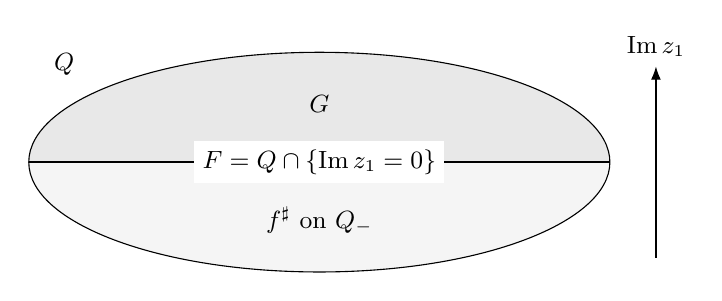
\begin{tikzpicture}[x=0.9cm,y=0.9cm,>=Latex,font=\small]
 \begin{scope}
  \clip (0,0) ellipse (4.1 and 1.55);
  \fill[black!4] (-4.2,-1.6) rectangle (4.2,0);
  \fill[black!9] (-4.2,0) rectangle (4.2,1.6);
 \end{scope}
 \draw (0,0) ellipse (4.1 and 1.55);
 \draw[thick] (-4.1,0) -- (4.1,0);
 \node[fill=white,inner sep=3pt] at (0,0)
       {$F=Q\cap\{\operatorname{Im}z_1=0\}$};
 \node at (0,0.82) {$G$};
 \node at (0,-0.82) {$f^\sharp$ on $Q_-$};
 \node at (-3.6,1.38) {$Q$};
 \draw[->] (4.75,-1.35) -- (4.75,1.35);
 \node[above] at (4.75,1.35) {$\operatorname{Im}z_1$};
\end{tikzpicture}
\caption{A schematic real section of the single-face enlargement;
passive variables are suppressed. The lower region carries $f^\sharp$
and the upper region carries $G$. The input maps are compared only on
a slightly enlarged real face $F$, with no prescribed complex collar
and no bound for $G$ away from the interface.}
\label{fig:real-interface}
\end{figure}


Choose small convex thickenings of \(Q\) and of \(P\).
Their lower sides, together with additional small neighborhoods,
can be kept in the domain of \(f\).  To verify this point without
a transversality assumption on the boundary of \(Q\), note that
as \(\eta\downarrow0\),
\[
 (Q+\eta\overline B)\cap\{\operatorname{Im}z_1\leq0\}
       \longrightarrow Q_-
\]
in the following sufficient sense: every sequence of points
in the left-hand sets has all its limit points in \(Q_-\).
Compactness then places these sets in any prescribed
neighborhood of \(Q_-\), for small \(\eta\).
Here \(\overline B\) is the Euclidean closed unit ball.

Lemma~\ref{loc:spray} gives a chart spray
\(f^\sharp(z,u,v)\) over a neighborhood of the thickened
lower side, with a fixed auxiliary polydisc in \(v\).
Its trace on
\[
 \{\operatorname{Im}z_1=0\}
\]
is holomorphic near a convex compact face in
\((t,y)=(\operatorname{Re}z_1,z_2,\ldots,z_n)\).
Apply Lemma~\ref{ana:face}, treating \(u,v\) as passive
polydisc variables.  We obtain an entire map \(G(z,u,v)\)
arbitrarily close to \(f^\sharp\), with, say, two tangential
derivatives on a slightly enlarged face and with fixed
smaller \(u,v\) margins.

On this interface, invert the vertical chart of \(f^\sharp\).
For a fixed smaller \(v\)-polydisc this produces a transition
\[
 \gamma(z,u,v)=v+c(z,u,v)
\]
between \(G\) and \(f^\sharp\), with \(c\) as small as desired
in the \(C^\alpha\) trace norm, for any fixed \(0<\alpha<1\).
This follows from the just obtained tangential derivative
accuracy and the bounded derivatives of the fixed chart
inverse on compact sets; Cauchy estimates on the retained
\(u\)-margin also give the required H\"older control in \(u\).
The transition is holomorphic in the complex tangential variables
and in \(v\).
Use \(f^\sharp\) on the lower side and \(G\) on the upper
side. Apply Lemma~\ref{glue:trace} with convex base \(Q\times P\),
normal coordinate \(z_1\), and only \(v\) as the fiber variable.
With losses smaller than the chosen thickening margins, it glues
their suitably reparametrized
central maps on a neighborhood of \(Q\times P\).
Its corrections can be made arbitrarily small on the lower
side, so the resulting map approximates \(f\) on \(Q_-\times P\).
No estimate for \(G\) away from the interface is used.

Finally let \(K\subset\C^n\) be any nonempty compact convex set,
and let \(f\) be given near \(K\times P\).
Thicken \(K\) and \(P\) slightly within this domain, and choose
a full-dimensional real convex polytope \(K'\) containing \(K\)
in its interior and still within the available thickening.
Choose a large coordinate polydisc \(\overline\Delta_R^{\,n}\)
containing \(K'\) in its interior.  Write
\[
 K'=\bigcap_{j=1}^M\{\ell_j(z)\leq b_j\},
\]
where the \(\ell_j\)'s are real linear forms, and remove these
constraints one at a time inside
\(\overline\Delta_R^{\,n}\).
At each stage both compact sets are convex, the old one has
nonempty interior, and a nonredundant constraint can be put
in the form \(\operatorname{Im}z_1\leq0\) by a complex affine
coordinate change.  The single-constraint argument therefore
extends the map approximately to the next compactum.
There are only finitely many stages, so assign their errors
a sum smaller than half the desired tolerance.
The final map is defined near
\(\overline\Delta_R^{\,n}\times P\), a polydisc.
Proposition~\ref{ana:polydisc} approximates it by an entire map,
using the remaining half of the tolerance.
This proves \({\cal A}_n\), completes the induction, and gives
Theorem~\ref{ana:cap} by taking no passive variables.
\end{proof}

\section{The projective case}\label{sec:projective}

We construct two complete directions from families of genus-one
curves. The curves on the K3 surface need not be smooth: the
complete flows take place on their smooth normalizations.

\begin{proposition}\label{prj:strips}
Let $S$ be a smooth projective complex K3 surface. There is a
nonempty Zariski open subset $U\subset S$ such that, for every
$x\in U$, there are $b>0$ and holomorphic maps
\[
\sigma_1:\C\times\Delta_b\longrightarrow S,\qquad
\sigma_2:\Delta_b\times\C\longrightarrow S
\]
which are locally biholomorphic at the origin and satisfy
\[
\sigma_1(0,0)=\sigma_2(0,0)=x,\qquad
\sigma_1(z,0)=\sigma_2(z,0)\quad (|z|<b).
\]
The complement $S\setminus U$ is algebraic of dimension at most
one. Consequently $S$ has property $L$ everywhere.
\end{proposition}

We use the genus-one case of the theorem of Chen and Gounelas
\cite[Theorem~A]{ChenGounelas}:
there are integral curves $C_n\subset S$ of geometric genus one
with $C_n^2\to\infty$, whose normalization maps belong to smooth
proper families of maps
\[
p_n:Y_n\longrightarrow T_n,\qquad q_n:Y_n\longrightarrow S.
\]
Here $T_n$ is an irreducible algebraic curve, the fibers of $p_n$
are connected genus-one curves, and the induced moduli map is
nonconstant. One fiber map is the normalization of $C_n$ followed
by its inclusion into $S$. A stable-map family includes, by definition,
a proper family of source curves; pulling back that family and restricting
to the smooth-source locus gives the proper maps $p_n$. No properness of
$T_n$ is asserted. We use the families over their full proper
fibers, even when evaluation is inverted only on a smaller open
subset.

\begin{lemma}\label{prj:prepare}
Let $S$ be a smooth projective integral surface, let $H$ be an
ample divisor, and let $p:Y\to T$ be a smooth proper family of
connected genus-one curves over a smooth irreducible algebraic
curve. Suppose that $q:Y\to S$ has nonconstant source-curve
moduli and that $q_{t_0}$ is the normalization map of an integral
curve $C\subset S$. After removing finitely many points of $T$,
every $q_t$ normalizes an integral image curve $C_t$ with
$H\cdot C_t=H\cdot C$. The evaluation map $q$ is dominant and
generically finite, and some nonempty Zariski open $V\subset S$
has finite etale surjective inverse image map $q^{-1}(V)\to V$.
\end{lemma}

\begin{proof}
The total space $Y$ is a smooth integral surface. Smoothness
follows from that of $p$ and $T$; connectedness follows from
connectedness of the base and fibers, and the irreducible
components of a smooth variety are disjoint open and closed
sets. Proper smooth local triviality shows that
$\deg(q_t^*H)$ is constant: it is the integral of $c_1(q^*H)$
on a fiber. At $t_0$ it equals $H\cdot C>0$. Thus all fiber
maps are nonconstant and finite onto their reduced integral
images.

Consider the graph map
\[
Q=(p,q):Y\longrightarrow T\times S.
\]
It is proper, by factoring through the closed graph in
$Y\times S$ followed by the proper map $p\times\mathrm{id}_S$,
and it has finite fibers. The proper quasi-finite criterion
therefore makes it finite. Its reduced image $Z$ is an integral
surface.
Choose a smooth point $z_0$ of $C$ and its unique preimage
$y_0\in Y_{t_0}$. The fiber $Q^{-1}(t_0,z_0)$ is a singleton.
Moreover $dQ_{y_0}$ is injective: a vector in its kernel is
vertical for $p$, and the normalization is an isomorphism near
$z_0$, so $dq$ is injective on that vertical tangent line.

The holomorphic constant-rank theorem embeds a small
neighborhood $W$ of $y_0$ in $T\times S$. Properness makes
$Q(Y\setminus W)$ closed in the analytic topology. Shrink a neighborhood
of $(t_0,z_0)$ to avoid that closed set and remain inside the
embedding chart. Thus $Q$ is an isomorphism over a nonempty
analytic open subset of $Z$. That subset meets the dense
Zariski open locus where the finite map is etale of its generic
degree. The degree is therefore one.

Since $Y$ is normal, $Q$ is the normalization of $Z$. Its
nonisomorphism locus $N\subset Z$ is closed of dimension at
most one. Remove the finitely many parameters of the vertical
curve components of $N$. Every horizontal component of $N$
has finite intersection with every remaining fiber, so the
irreducible support
$|Z_t|=q_t(Y_t)$ is not contained in $N$. The restriction $q_t$
is consequently finite and birational onto its reduced image
$C_t$, hence is its normalization. The projection formula gives
\[
H\cdot C_t=\deg(q_t^*H)=H\cdot C.
\]

If the closure of $q(Y)$ were a curve, each retained fiber map
would normalize that same integral curve. Their smooth source
curves would all be isomorphic, contrary to nonconstant moduli.
Thus $q$ dominates $S$. Source and target have dimension two,
so the induced function-field extension is finite and, in
characteristic zero, separable.

Here the desired finite etale locus must be justified even
though $q$ itself is not assumed proper. Choose affine opens
$V_0=\operatorname{Spec}B\subset Y$ and
$U_0=\operatorname{Spec}A\subset S$ with $q(V_0)\subset U_0$.
Every one of finitely many $A$-algebra generators of $B$ is
algebraic over $\operatorname{Frac}A$. Invert a common nonzero
element of $A$ to make their monic equations integral; the
resulting affine map is finite. Remove also the closure of
$q(Y\setminus V_0)$, of dimension at most one, and shrink to
the etale locus. This leaves a nonempty Zariski open $V$ on
which the full inverse image is the finite etale piece.
It is surjective because it is finite and dominant.
\end{proof}

Normalize the parameter curves supplied by Chen--Gounelas,
retaining a point above each specified normalization fiber,
and pull back the families. The bases are then smooth
irreducible curves; smoothness, properness, and nonconstant
moduli persist. Fix a very ample divisor $H$ on $S$. The
Hodge index inequality
\[
(H\cdot C_n)^2\ge H^2 C_n^2
\]
shows that the ample degrees are unbounded.
Choose two distinct degrees $d_1,d_2$ and apply
Lemma~\ref{prj:prepare}. We obtain two families
\[
p_i:Y_i\longrightarrow T_i,\qquad q_i:Y_i\longrightarrow S
\quad(i=1,2)
\]
whose fiber maps normalize integral curves of degree $d_i$.
Choose a common nonempty open $V\subset S$ on which
$Y_i^V=q_i^{-1}(V)\to V$ are both finite etale and surjective.
Only their inverse sheets are restricted to $V$: the maps
$q_i$ remain defined on all of $Y_i$.

\begin{lemma}\label{prj:transverse}
There is a nonempty Zariski open $U\subset V$ such that any
two lifts $y_i\in Y_i^V$ of a point $x\in U$ have distinct
transported vertical tangent lines
\[
dq_1\bigl(\ker(dp_1)_{y_1}\bigr)
\ne dq_2\bigl(\ker(dp_2)_{y_2}\bigr)
\quad\text{in }T_xS.
\]
The closure in $S$ of the exceptional locus has dimension
at most one.
\end{lemma}

\begin{proof}
Form the finite etale cover
\[
W=Y_1^V\times_VY_2^V\xrightarrow{\,Q\,}V,\qquad
\tau_i=p_i\circ\operatorname{pr}_i.
\]
Every irreducible component of the smooth surface $W$
dominates $V$, since a finite etale map is both open and closed.
The maps $\tau_i$ are submersions. Their algebraic rank-drop
locus
\[
I=\{d\tau_1\wedge d\tau_2=0\}
\]
records equality of the transported vertical directions.

No component of $W$ can be contained in $I$. If one were,
identify a small analytic neighborhood in it with an open
subset of $S$ using $Q$. In a coordinate $s=\tau_1$,
dependence of the differentials makes $\tau_2$ depend only on
$s$. A local $\tau_1$-fiber would then lie in a local
$\tau_2$-fiber. Its nonconstant image germ in $S$ lies in an
integral curve from each family. Two distinct integral curves
on a projective surface have finite intersection, so the
curves must coincide. This contradicts their distinct
$H$-degrees.

Consequently $\dim I\le1$. Since $Q$ is finite, $Q(I)$ is
closed in $V$ and has dimension at most one; its algebraic
closure in $S$ has the same dimension bound. Taking
\[
U=S\setminus\bigl((S\setminus V)\cup\overline{Q(I)}^{\,S}\bigr)
\]
proves all assertions.
\end{proof}

\begin{lemma}[Complete vertical flows]\label{prj:flow}
Let $p:Y\to\Delta$ be a proper holomorphic submersion with
connected genus-one fibers. After shrinking the base disc,
there is a nowhere-zero holomorphic vertical vector field
whose flow is jointly holomorphic for all complex times.
Its restriction to the central fiber may be prescribed as
any nonzero holomorphic vector field there.
\end{lemma}

\begin{proof}
For every fiber $C$, the space $H^0(C,T_C)$ is one-dimensional
and its nonzero elements have no zeros. The relative tangent
bundle is locally free and flat over the base. Grauert's
cohomology and base-change theorem \cite[\S~7, Satz~5]{Grauert} makes
$p_*T_{Y/\Delta}$ a holomorphic line bundle with these spaces
as fibers. The evaluation morphism
\[
p^*(p_*T_{Y/\Delta})\longrightarrow T_{Y/\Delta}
\]
is an isomorphism on every fiber, hence everywhere.
A local frame gives the vertical field, and scaling it
prescribes its central restriction.

Take a smaller closed base disc. Its full inverse image is
compact. Local holomorphic flow existence and a finite cover
of this compact set give a common time radius $\epsilon>0$.
The flow preserves fibers, so successive small-time flows
remain in the same compact inverse image. Composing the
time-$z/M$ flow $M$ times defines a holomorphic flow for
$|z|<M\epsilon$. Uniqueness and the local group law make
these extensions agree as $M$ increases. They define the
jointly holomorphic flow for every $z\in\C$ over the smaller
open base disc.
\end{proof}

\begin{proof}[Proof of Proposition~\ref{prj:strips}]
Fix $x\in U$ and lifts $y_i$ as in Lemma~\ref{prj:transverse}.
Use Lemma~\ref{prj:flow} on each full proper family over a
small base disc about $p_i(y_i)$. Let $\xi_i$ be the resulting
vertical fields and $\operatorname{Fl}_i^z$ their complete
flows. Then
$v_i=dq_i(\xi_i(y_i))$ are independent tangent vectors at $x$.

Choose a local section $e_1(w)$ of $p_1$ through $y_1$ and set
\[
\sigma_1(z,w)=q_1\bigl(\operatorname{Fl}_1^z(e_1(w))\bigr).
\]
This map is defined for all $z\in\C$ and all sufficiently
small $w$. It is locally biholomorphic at the origin:
the flow derivative is vertical, the section derivative
projects nontrivially to the base, and $q_1$ is etale at $y_1$.
Put $\varphi(z)=\sigma_1(z,0)$.

For small $z$ lift $\varphi(z)$ through the local inverse
of $q_2$ at $y_2$, obtaining a holomorphic map $\ell_2(z)$
with $q_2(\ell_2(z))=\varphi(z)$. Shrink its domain so
$p_2(\ell_2(z))$ lies in the disc supporting the second
complete flow, and define
\[
\sigma_2(z,w)=q_2\bigl(\operatorname{Fl}_2^w(\ell_2(z))\bigr).
\]
It is defined for small $z$ and every $w\in\C$.
Its derivatives at the origin are $v_1,v_2$, so it too
is locally biholomorphic. At time zero it returns its
starting point, giving the exact identity
$\sigma_2(z,0)=\varphi(z)=\sigma_1(z,0)$.
Choose a common radius for the bounded variables.
The inverse sheet was used only for the initial lift;
subsequent flow values lie in entire proper fibers,
where $q_2$ is still defined.

Proposition~\ref{loc:criterion} gives $L$ throughout $U$.
Its algebraic complement has dimension at most one, so
Corollary~\ref{loc:disc} gives $L$ at the remaining points.
\end{proof}


\section{Exact symplectic sewing of annular chains}
\label{sew:section}

This section isolates the analytic construction needed in the geometric
arguments.  The domains are cylinders, not discs.  Consequently, a closed
holomorphic one-form on an overlap need not be exact.  Its period is the
obstruction that must be removed before the iteration can converge.

Put $\mathcal C=\C/\Z$, and write $Y=\operatorname{Im}w$ on
$\mathcal C$.  We use the form
\[
                 \omega_0=dw\wedge dp
\]
on products of $\mathcal C$ with a parameter disc.  A symplectic map
$F=(W,P)$ between such products is called \emph{exact} if
\[
                F^*(P\,dW)-p\,dw
\]
is an exact holomorphic one-form.  Since a cylinder times a disc has first
homology $\Z$, this is equivalent to the vanishing of its integral around
one positively oriented period circle.  All lifts below have degree one:
$W(w+1,p)=W(w,p)+1$ and $P(w+1,p)=P(w,p)$.

\begin{theorem}[Annular-chain sewing]\label{sew:chain}
Let $M$ be a complex surface with a nowhere-zero holomorphic two-form
$\omega$.  Fix $0<h<1/8$, $r>0$, and $A<\infty$.  For each $j\in\Z$,
let $L_j\geq1$ and let
\[
 \phi_j:\{ -2h<Y<L_j+2h\}\times\Delta_r\longrightarrow M
\]
be a holomorphic map with $\phi_j^*\omega=\omega_0$.  Suppose there are
holomorphic translations
\[
 J_j(w,p)=(w+a_j(p),p),\qquad
 |\operatorname{Im}a_j(p)+L_j|<h/8,\qquad |a_j'(p)|\leq A,
\]
and exact symplectic transitions $F_j$ on
\[
 S_j(h,r)=\{|Y-L_j|<h\}\times\Delta_r
\]
such that $\phi_j=\phi_{j+1}\circ F_j$.  Write
\[
                  J_j^{-1}F_j=(w+u_j,p+v_j).
\]
Assume these lifts exist and
$\sup_j\|(u_j,v_j)\|_{S_j(h,r)}\leq e$.

There are $b>0$ and $e_*>0$, depending only on $h,r,A$ and the indicated margins,
such that, if $e<e_*$, these charts give a holomorphic symplectic
immersion
\[
                  \Phi:\C\times\Delta_b\longrightarrow M
\]
which is periodic of period one in the first variable.
On a smaller domain in every original block, with fixed positive
margins at both ends, $\Phi$ is obtained from $\phi_j$ by a small
periodic symplectic change of variables.  The corrected transitions are
\[
        (w,p)\longmapsto(w+\widetilde a_j(p),p).
\]
The changes of variables and $\widetilde a_j-a_j$, together with any
fixed finite number of derivatives on further smaller domains, tend
uniformly to zero as $e\to0$.  None of these assertions requires an
upper bound for the $L_j$ or a bound on the number of blocks.
\end{theorem}

Here and below $\Delta_r=\{p\in\C:|p|<r\}$; a norm on a noncompact
cylinder is the supremum norm of a periodic function.  We give the
estimates and the domain construction explicitly.

\subsection{Domains and the infinitesimal obstruction}

For a current collection of translations, define
\[
\begin{split}
 S_j(s,\rho)&=\{|Y-L_j|<s,\ |p|<\rho\},\\
 D_j(s,\rho)&=\{L_{j-1}-s<Y-\operatorname{Im}a_{j-1}(p),\quad
                         Y<L_j+s,\quad |p|<\rho\}.
\end{split}
\]
The lower edge of $D_j$ is near height zero.  The particular slanted
lower edge is useful: the lower inequality for $D_{j+1}$, after
composition with $J_j$, is precisely $Y>L_j-s$.  Thus $S_j$ lies in
$D_j$, and its translate lies in $D_{j+1}$.  The other two inequalities
have a fixed buffer because $L_j\geq1$ and $s<1/8$.

If $s$ and $\rho$ are each decreased by $\delta$, then the smaller
$D_j$ admits coordinate Cauchy discs of radius at least
$c\delta/(1+A)$ in the larger $D_j$.  The same assertion holds for
seams and for their translated copies.  This follows directly from
\[
 |a_j(p')-a_j(p)|\leq A|p'-p|.
\]
In particular, all fixed-order Cauchy bounds cost only a fixed power
of $\delta^{-1}$, independently of $j$ and $L_j$.  In the estimates
below constants may depend on $h,r,A$ and on fixed fractions of the
initial margins; we take $0<\delta<1$.

\begin{lemma}[Removal of the transverse zero mode]\label{sew:linearize}
Suppose $E=(w+u,p+v)$ is exact symplectic on a seam and
$\|(u,v)\|\leq e$.  After a margin loss $\delta$ there are a
holomorphic function $u_0(p)$ and a periodic mean-zero function $H$
such that
\[
 (u,v)=(u_0,0)+X_H+R,\qquad
 X_H=(H_p,-H_w),\qquad
 \|H\|\leq Ce,\quad \|R\|\leq C\delta^{-2}e^2.
\]
Here $u_0$ is the zero Fourier coefficient of $u$.
\end{lemma}

\begin{proof}
Symplecticity and exactness respectively give
\begin{align}
 u_w+v_p&=-u_wv_p+u_pv_w,\label{sew:symplectic-error}\\
 0&=\int_0^1 v(w,p)(1+u_w(w,p))\,dw.
                                      \label{sew:period-error}
\end{align}
The second identity follows by expanding
$(p+v)d(w+u)-p\,dw$ on a horizontal period circle; the integral of
$p u_w$ is zero.  Consequently its mean $v_0(p)$ satisfies
\[
                  |v_0(p)|\leq C\delta^{-1}e^2.
\]
Take the unique mean-zero periodic primitive satisfying
\[
                        H_w=-v+v_0.
\]
Integration along one horizontal period, followed by subtraction of
the mean, bounds $H$ by $Ce$.  This primitive is holomorphic in $p$.
Equation~\eqref{sew:symplectic-error} gives
\[
 \partial_w(u-H_p)=-u_wv_p+u_pv_w-v_0'(p).
\]
The right side has zero mean and is $O(\delta^{-2}e^2)$ after one
additional fixed fraction of the margin loss.  Integrating its
mean-zero primitive bounds $(u-H_p)-u_0$ by the same quantity.
The other component of $R$ is $v_0$.  Rescaling the allocation of
$\delta$ among these finitely many steps proves the stated estimate.
\end{proof}

The role of exactness is now visible.  Without
Equation~\eqref{sew:period-error}, the first-order constant term in
$v$ need not vanish.  It cannot be absorbed into a translation that
preserves the common transverse coordinate.

\subsection{A uniformly bounded Fourier splitting}

\begin{lemma}[Splitting along the whole chain]\label{sew:split}
Suppose the periodic functions $H_j$ have mean zero, are holomorphic
on $S_j(s,\rho)$, and have norm at most $e$.  Assume
\[
                 |\operatorname{Im}a_j+L_j|\leq\kappa<1/4.
\]
There are periodic holomorphic functions $G_j$ on
$D_j(s-\delta,\rho)$ satisfying
\begin{equation}\label{sew:split-equation}
                  G_j-G_{j+1}\circ J_j=-H_j.
\end{equation}
on the smaller seams.  Their bounds, on domains with the appropriate
additional losses, are
\[
 \|G_j\|\leq C\delta^{-1}e,\qquad
 \|X_{G_j}\|\leq C\delta^{-2}e,\qquad
 \|DX_{G_j}\|\leq C\delta^{-3}e.
\]
All constants are uniform in the block lengths and the number of
blocks.
\end{lemma}

\begin{proof}
Set $T_j=-H_j$ and write
\[
             T_j(w,p)=\sum_{n\neq0}t_{j,n}(p)e^{2\pi i n w}.
\]
The coefficients are holomorphic in $p$.  Denote the negative and
positive parts by $T_j^-$ and $T_j^+$.  Starting from $(w_j,p)$,
continue the coordinates by
\[
                          w_{s+1}=w_s+a_s(p)
\]
in either direction, and define
\begin{equation}\label{sew:fourier-sum}
 G_j(w_j,p)=\sum_{l\geq j}T_l^-(w_l,p)
                         -\sum_{l<j}T_l^+(w_l,p).
\end{equation}
For negative coefficients use a horizontal coefficient-bound line
at height $L_l+s-\delta/4$.  An evaluation point of
$D_j(s-\delta,\rho)$ is below that line, in the continued $l$-th
coordinate, by at least
\[
                     3\delta/4+(1-\kappa)(l-j)
                     \qquad(l\geq j).
\]
For positive coefficients use height $L_l-s+\delta/4$.  The
evaluation point is above that line by at least
\[
                     3\delta/4+(1-\kappa)(j-1-l)
                     \qquad(l<j).
\]
For the nearest terms these inequalities are exactly the two defining
inequalities for $D_j$.  For each further term an intervening block
contributes at least $1-\kappa$.

The absolute value of a Fourier mode is
$|e^{2\pi i n w}|=e^{-2\pi nY}$.  Therefore both sums, including the
sum over frequencies, are bounded by a constant times
\[
 e\sum_{n\geq1}\sum_{q\geq0}
       \exp\bigl(-2\pi n(3\delta/4+(1-\kappa)q)\bigr)
 \leq C e\delta^{-1}.
\]
This proves normal convergence and holomorphicity, including in the
parameter.  Telescoping Equation~\eqref{sew:fourier-sum} leaves
$T_j^-+T_j^+=-H_j$, proving
Equation~\eqref{sew:split-equation}.  Cauchy estimates on smaller
$D_j$ give the derivative bounds.  In particular, one need not
differentiate a sum of an unbounded number of translation functions
term by term.
\end{proof}

\subsection{The nonlinear iteration}

We record the domain issues in the Newton step.  Reserve a fixed
number of successive margin losses, each comparable to $\delta$,
for the primitive, Fourier splitting, derivative estimates, flows,
and composition.  Enlarging this fixed number if necessary does not
depend on any block length.  In the following statements the total
loss is denoted by $c_0\delta$, with $c_0$ a fixed constant.

Apply Lemma~\ref{sew:linearize} to $E_j=J_j^{-1}F_j$, and then
Lemma~\ref{sew:split}.  Let $K_j$ be the time-one map of $X_{G_j}$.
It is defined on the reserved smaller $D_j$ provided
$C\delta^{-2}e<\delta$.  Its displacement and first-order remainder
satisfy
\begin{equation}\label{sew:flow-estimates}
 \|K_j-\operatorname{id}\|\leq C\delta^{-2}e,\qquad
 \|K_j-\operatorname{id}-X_{G_j}\|
                              \leq C\delta^{-5}e^2.
\end{equation}
Indeed the second estimate follows by integrating the differential
equation for the flow and using
$\|DX_{G_j}\|\,\|X_{G_j}\|\leq C\delta^{-5}e^2$.
Negative-time flows satisfy the same estimates on the corresponding
smaller domains.

The new transition and its proposed model are
\[
 F_j^{\mathrm{new}}=K_{j+1}^{-1}F_jK_j,\qquad
 J_j^{\mathrm{new}}(w,p)=(w+a_j(p)+u_{j,0}(p),p).
\]
To check the cancellation without differentiating a long coordinate
change, put $Q_j=G_{j+1}\circ J_j$.  The conjugate
$J_j^{-1}K_{j+1}J_j$ is the time-one Hamiltonian flow of $Q_j$.
On a buffered seam $\|Q_j\|\leq C\delta^{-1}e$; the same Cauchy
and flow estimates apply to it.  The linear term of
\[
        J_j^{-1}K_{j+1}^{-1}J_j\, E_j\, K_j
\]
is
\[
 (u_j,v_j)+X_{G_j}-X_{Q_j}
            =(u_{j,0},0)+R_j.
\]
Here the Hamiltonian terms cancel by
Equation~\eqref{sew:split-equation}.  The remaining products are
quadratic: Equation~\eqref{sew:flow-estimates} bounds the flow
remainders by $C\delta^{-5}e^2$, and the other composition errors
are bounded by a first derivative times a displacement.  For example,
they are bounded by
\[
 C(\delta^{-1}e)(\delta^{-2}e)
       \quad\hbox{or}\quad
 C(\delta^{-3}e)(\delta^{-2}e).
\]
Finally compose with $(w,p)\mapsto(w-u_{j,0}(p),p)$ to normalize
by $J_j^{\mathrm{new}}$.  Its derivative differs from the identity
by at most $C\delta^{-1}e$ and introduces only another quadratic
term.  It follows, for some fixed integer $q\geq6$, that
\begin{equation}\label{sew:newton-bound}
 \sup_j\|(J_j^{\mathrm{new}})^{-1}F_j^{\mathrm{new}}
                                     -\operatorname{id}\|
                              \leq C\delta^{-q}e^2.
\end{equation}
One can use the displayed estimates with $q=6$; allowing a larger
fixed $q$ absorbs harmless reallocations of the margins.  No
operation in this step involves more than two adjacent charts.

The new left boundary of $D_j$ changes by at most
$\|u_{j-1,0}\|\leq e$.  Flow displacements are
$O(\delta^{-2}e)$.  Hence all new domains, translated seams and
inverse-flow domains fit in their reserved predecessors when
$C\delta^{-q}e$ is sufficiently small compared with $\delta$.
The model derivative changes by at most $C\delta^{-1}e$.
These observations justify both the domain inclusions used above and
their uniform repetition.

Exactness persists.  With $\lambda=p\,dw$, Cartan's formula for our
Hamiltonian convention gives
\[
                  \mathcal L_{X_H}\lambda=d(pH_p-H).
\]
Thus the flows are exact.  The shear $J_j$ is exact because
$J_j^*\lambda-\lambda=p a_j'(p)\,dp$ has a holomorphic primitive
on the parameter disc.  Compositions and inverses of exact maps are
exact.

\begin{proof}[Proof of Theorem~\ref{sew:chain}]
Start with slightly smaller $s_0<h$ and $\rho_0<r$.  Fix a small
$d_0>0$ and take $\delta_n=d_0 2^{-n}$.  Choose $d_0$ so that
\[
 c_0\sum_{n\geq0}\delta_n
                   <\tfrac14\min(s_0,\rho_0).
\]
At stage $n$ reduce both margins by $c_0\delta_n$.  Thus their
limits remain positive.  Set $B=C d_0^{-q}$, increasing the uniform
constant in Equation~\eqref{sew:newton-bound} once if needed.  If
$e_n$ bounds the normalized errors, then
\[
 e_{n+1}\leq B2^{qn}e_n^2.
\]
For $x_n=B2^{q(n+1)}e_n$ this becomes $x_{n+1}\leq x_n^2$.
Consequently, if $x_0\leq\theta<1$, then
\[
 e_n\leq B^{-1}2^{-q(n+1)}\theta^{2^n}.
\]
Every series $\sum_n\delta_n^{-k}e_n$, with fixed $k$, converges
and tends to zero as $e_0\to0$.  Taking $e_0$ still smaller ensures
all the margin conditions above, keeps
$|\operatorname{Im}a_j^{(n)}+L_j|<h/3$, and keeps the translation
derivative bound below $A+1$.  These estimates are uniform in $j$.

The successive compositions of the $K_j$ converge uniformly, with
derivatives on smaller domains, to maps $C_j$ into the original
block domains.  To see this directly, sum their displacements;
their derivative norms are bounded by a convergent product of
$1+C\delta_n^{-3}e_n$.  The reserved inclusions keep every
composition in its domain.  The limits remain symplectic because
their differentials converge and each determinant is one.  Put
$\widetilde\phi_j=\phi_j\circ C_j$ and
$\widetilde a_j=\lim_n a_j^{(n)}$.  Passing to the limit in the
chart identities on the seams gives
\[
 \widetilde\phi_j(w,p)=
       \widetilde\phi_{j+1}(w+\widetilde a_j(p),p).
\]
The parameter radius has been decreased by the fixed sum of reserved
losses and is still bounded below by a positive number depending only
on the initial margins. A smaller common radius $b$ can therefore be
fixed before the error threshold, independently of the chain.

It remains to identify the domain, rather than invoke a
uniformization theorem.  Fix block zero, put $w_0=w$, and define
$w_{j+1}=w_j+\widetilde a_j(p)$ in both directions.  These are
holomorphic shears, and $dw_j\wedge dp=dw\wedge dp$.  Use the
$j$-th chart between the heights
\[
       \operatorname{Im}w_{j-1}=L_{j-1},\qquad
       \operatorname{Im}w_j=L_j,
\]
including the surviving overlaps.  In $w_j$ coordinates the first
height is near zero and the second is $L_j$.  Their separation is
at least $1-h/3$.  Hence the successive edges tend to both
infinities, locally uniformly in $p$, and the charts cover all of
$\C\times\Delta_b$.  They agree on overlaps by the limiting
identity.  Their common pullback form is $dw\wedge dp$, proving
immersion.  Periodicity follows from the periodicity of the original
charts and every correction.  The summable estimates also prove
the claimed approximation statements.
\end{proof}

\subsection{Enforcing exactness by recentering}

The geometric applications supply nearly matching blocks, but not
initially exact transitions.  The following observation explains
precisely how their centers are allowed to move.

\begin{lemma}[Period adjustment]\label{sew:centers}
Suppose symplectically normalized charts, together with corresponding
model charts, are available for centers varying in larger transverse
discs.  Suppose the actual charts are uniformly close to their
models, and transitions at matching model positions are uniformly
close to degree-one shears.  The transition into a newly added block
can be made exact by a transverse translation of that block of size
bounded by its transition error.  Recenter its model by the same
translation.  The approximation of that block by its own recentered
model retains its original bound.

Consequently, such adjustments can be repeated indefinitely whenever
the updated centers remain in a region with uniform buffered chart
choices.  No bound on their accumulated displacement relative to
the first center is required.
\end{lemma}

\begin{proof}
For a transition $F=(W,P)$ the closed one-form
$P\,dW-p\,dw$ has a constant complex period
\[
                     D=\int(P\,dW-p\,dw).
\]
It is independent of the representative period circle and of $p$.
Evaluation at an interior circle with $p=0$, using Cauchy estimates
on a fixed seam margin, bounds $|D|$ by the error from a shear.
Replace the added target chart by
$(W,P_{\rm new})\mapsto\phi(W,P_{\rm new}+D)$.  The transition
now has $P_{\rm new}=P-D$, so its period is
\[
        D-D\int dW=0.
\]
The last integral is one because the transition has degree one.
In a backward extension one instead translates the newly added
input chart, with the corresponding sign.  Uniform buffers permit
these small translations.

Apply the identical substitution to the model chart.  Its outgoing
end is now the outgoing end of that updated model, and this is the
position used to choose the following block.  Both actual and
model maps were defined on a larger disc, so their difference after
restriction and translation has the same uniform bound.  The old
seam still has only a small error; the assertion does not require
the two moved model centers to coincide there.  Repeating this
argument compares each new chart with its current model and never
sums the previous matching errors.
\end{proof}

For completeness, the normalization used in this lemma is compatible
with periodicity.  If a nearby chart pulls back the surface form to
$k(w,t)\,dw\wedge dt$, with $k$ periodic and close to one, put
\[
                       p(w,t)=\int_0^t k(w,s)\,ds.
\]
Then $dw\wedge dp=k\,dw\wedge dt$, and $(w,t)\mapsto(w,p)$ is a
small periodic biholomorphic change on smaller domains.  Its inverse
is obtained uniformly with margins.  Additive origins in $w$ may
also be changed by holomorphic functions of $p$; these changes are
exact shears, so they do not affect the period adjustment.

\section{An open region of K3 periods}
\label{deg:section}

Theorem~\ref{sew:chain} permits the centers of successive annuli to
move.  We now construct a degeneration for which every possible new
center admits another block.  This is the reason an infinite chain
can be continued after the exactness adjustments.

\begin{proposition}\label{deg:open}
There is a nonempty open subset of the full marked K3 period domain
such that every surface with period in this subset has property $L$
at every point.
\end{proposition}

The openness here is unrestricted: the nearby surfaces need not be
projective.  We shall first produce one smooth quartic with a finite
collection of buffered chart constructions, then deform all those
constructions to its full local deformation space.

\subsection{The semistable model and its regular pencils}

Choose two general smooth quadrics $Q_+,Q_-\subset\mathbb P^3$.
Their intersection $E$ is a smooth elliptic quartic.  For a general
quartic form $G$ consider the family
\begin{equation}\label{deg:quartic-family}
                         Q_+Q_-=\alpha G.
\end{equation}
Here the same symbols $Q_+,Q_-$ denote their quadratic equations.
The sixteen zeros $Z$ of $G|_E$ are simple.  Near such a zero the
total space has equation $xy=\alpha t$, up to holomorphic changes
of coordinates.  Blowing up one component, locally the ideal
$(x,\alpha)$, is a small resolution.  For example, in one chart
write $\alpha=xa$; the strict transform has $y=at$ and the map to
the parameter disc is $\alpha=xa$.  In the other chart write
$x=\alpha b$; the equation becomes $t=by$, with smooth coordinates
$(\alpha,b,y)$ and projection $\alpha$.  Thus the resolved total
space is smooth and the central fiber has normal crossings.

Its two components, with a suitable choice of labels, are a quadric
$S^+$ and the blowup $S^-$ of a quadric at $Z$; they meet along the
strict transform of $E$, again denoted $E$.  The resolution is
crepant because it is small and the original hypersurface is
Gorenstein.  Adjunction for the quartic family supplies a nowhere-zero
relative dualizing form.  On $S^\pm$ it becomes a logarithmic
symplectic form $\omega_\pm$ with simple pole along $E$ and opposite
nonzero residues.  In a normal-crossing chart we have
\begin{equation}\label{deg:neck-form}
       uv=\alpha,\qquad
       \omega_\alpha=k(u,v,t)\,\frac{du}{u}\wedge dt,
\end{equation}
where $k$ is holomorphic and nowhere zero and $t$ is a coordinate
along $E$.  In particular $k(0,0,t)dt$ is its residue on the
$u$-component; the residue on the $v$-component is its negative.
For small nonzero $\alpha$, the fibers of
Equation~\eqref{deg:quartic-family} are smooth quartic K3 surfaces.

Call a fiber of a base-point-free pencil on $S^+$ or $S^-$
\emph{regular} if it is a smooth rational curve, the pencil map is
smooth along it, and it meets $E$ transversely at two distinct
points.  We use the two ruling pencils, pulled back on $S^-$, and
on $S^-$ also the pencils of $(1,1)$ curves through two distinct
points of $Z$, with their two base points subtracted.

\begin{lemma}\label{deg:regular-pencils}
The quadrics and $G$ can be chosen so that:
\begin{enumerate}
 \item Through every point of $E$ on each component there is a
       regular fiber of one of these finitely many pencils.
 \item The union of their regular fibers contains the complement
       of a proper algebraic subset of each component.
 \item Every regular fiber has, away from $E$, a transverse
       intersection with a regular fiber of another pencil.
\end{enumerate}
\end{lemma}

\begin{proof}
On a plain quadric, identify the two rulings with the projections
of $\mathbb P^1\times\mathbb P^1$.  Their restrictions to $E$ have
degree two.  They cannot both ramify at one point: otherwise the
differential of the inclusion of the smooth curve $E$ in the
quadric would vanish.  This proves the first assertion on $S^+$.

For the blown-up quadric, a ruling fiber is additionally forbidden
when it passes through a point of $Z$.  Choose $Z$ generally so
that its points avoid both ruling ramification sets, and so
that a forbidden level of one ruling and a forbidden level of the
other have a common point on $E$ only at a point of $Z$.  To check
that these are proper conditions, write the two projections as
$\pi_1,\pi_2$.  Their ramification sets are disjoint.  Conditions
involving one ramification set and one $\pi_i(Z)$ exclude only
finitely many values for the corresponding point of $Z$.  For
distinct $z_i,z_j$, the condition that the grid point with
coordinates $(\pi_1(z_i),\pi_2(z_j))$ lie on $E$ is a proper
condition on the pair.  For $i=j$ the grid point is $z_i$ itself.
Thus, away from $Z$, at least one ruling remains regular.

Fix $z_i\in Z$.  Choose another center $z_j$ and take the plane
through the tangent line to $E$ at $z_i$ and through $z_j$.  For
general choices its intersection with the quadric is a smooth
$(1,1)$ curve.  Its divisor on $E$ is
\[
                        2z_i+z_j+z_k,
\]
with $z_k$ different from $z_i,z_j$, and it passes through no other
point of $Z$.  Its strict transform is a member of the pencil of
$(1,1)$ curves through $z_i,z_j$.  The chord through these two
points is not a ruling line; hence the pencil has exactly these
two simple base points, which are resolved by the blowups.  An
order-two contact at $z_i$ becomes a simple transverse
intersection with the strict transform of $E$.  The simple
intersection at $z_j$ disappears, and the intersection at $z_k$
remains.  The selected strict transform is therefore a regular
fiber through the point of $E$ over $z_i$.

All the generic requirements just used are simultaneous finite
proper conditions.  More explicitly, on the elliptic curve the
residual $z_k$ is determined by the hyperplane divisor class and
$2z_i+z_j$; excluding coincidences or another center imposes a
proper condition on at most three of the centers.  The other
requirements involve at most two centers and fixed branch data.
The divisor $Z$ ranges over the complete degree-sixteen linear
system $|\mathcal O_E(4)|$.  Indeed the restriction of quartic
forms is surjective, as follows from the Koszul resolution for
the intersection of two quadrics.  In an ordered general divisor
of this degree any specified fewer than sixteen points vary
freely; the remaining points satisfy the one elliptic sum
condition.  Hence the finitely many proper conditions above can
all be avoided.

For each of the finitely many pencils, only finitely many members
fail to be smooth or meet $E$ nontransversely.  Their union is a
proper algebraic set, proving the second assertion.  Finally, on
any regular rational fiber, at least one of the two ruling
projections is nonconstant.  This is immediate for a ruling fiber
by using the other ruling; for a $(1,1)$ fiber both projections are
nonconstant.  Away from finitely many points of the fiber the
corresponding ruling member is regular and the projection has
nonzero derivative.  Such an intersection is transverse and can
be chosen off $E$.
\end{proof}

We now make finite compact choices, each with an open buffer.
Let $G_{\rm reg}$ be the union of \emph{all} regular fibers from
the listed pencils.  Its complement is contained in a proper
algebraic set, and $G_{\rm reg}$ contains a neighborhood of $E$.
By the first assertion of Lemma~\ref{deg:regular-pencils}, compact
subfamilies of regular fibers supply entries at every point of
$E$.  By its third assertion each required family can, after
restriction, be equipped with a transverse partner at an
interior point, with a positive transversality margin in local
charts.  Compactness supplies finitely many such choices near
$E$.

For each point of the algebraic exceptional set away from $E$,
choose a coordinate line not contained in that set and a small
radius whose boundary avoids it.  The boundary then lies in
$G_{\rm reg}$.  Small translations and tilts retain this boundary
containment, so the disc construction supplies a neighborhood of
possible centers.  Points of $G_{\rm reg}$ themselves have regular
coordinate neighborhoods.  On the compact region outside a
chosen neighborhood of $E$, finitely many of these two kinds of
center neighborhoods suffice.  Only after choosing these finitely
many discs do we add finitely many regular patches covering their
compact boundaries, along with the corresponding regular
families and transverse partners.  Thus every retained datum
belongs to a finite buffered collection.  The algebraic
exceptional set is used before the finite selection.  These
disc choices will be used with
Corollary~\ref{loc:disc} after constructing the strips.

\subsection{Core and neck coordinates}

\begin{lemma}\label{deg:core-coordinates}
On a small parameter disc of any compact regular family there are
coordinates $(z,p)\in\mathbb P^1\times\Delta_r$ in which the two
ends are $z=0,\infty$ and
\[
              \omega_\pm=\frac{1}{2\pi i}\frac{dz}{z}\wedge dp.
\]
Either end can be designated as the entrance.  With entrance at
$\infty$, exit at $0$, and $z=c\exp(2\pi i w)$, this reads
$\omega_\pm=dw\wedge dp$.  The parameter $p$ is a local affine
coordinate for either end position on $E$, read using its signed
residue differential.
\end{lemma}

\begin{proof}
Over a small disc the smooth proper family of rational fibers is
a holomorphic $\mathbb P^1$ bundle and is trivial there.  One can
see this by choosing a local section, taking its relative
degree-one line bundle, and using sections and base change to
identify the family with a projective bundle.  The two distinct
end sections can then be put at zero and infinity.

In a parameter $s$ on this disc write the logarithmic form as
$f(z,s)dz\wedge ds$.  For each $s$, the one-form
$f(z,s)dz$ on $\mathbb P^1$ has only simple poles at zero and
infinity.  It is therefore $b(s)dz/z$.  Nondegeneracy makes $b$
nonzero.  Set $dp=2\pi i b(s)ds$.

Let $t_+(s)$ and $t_-(s)$ be the exit and entrance positions on
$E$, and let $\rho$ be the residue differential on this
component.  Taking residues gives the exact identities
\[
             dp=2\pi i\,t_+^*\rho=-2\pi i\,t_-^*\rho.
\]
They also follow from the constancy of the elliptic sum of the
two intersection points.  Since both ends are transverse,
$t_+$ and $t_-$ are locally invertible.  Thus $p$ moves each
end freely and the stated residue interpretation follows.
\end{proof}

In a fixed normal-crossing chart at an end, its nonzero normal
coordinate on the corresponding central component has the
uniform expansions
\begin{align}
 u&=k_-(p)z^{-1}\bigl(1+O(z^{-1})\bigr)
                                    &&\text{at the entrance},
                                      \label{deg:entrance}\\
 u&=k_+(p)z\bigl(1+O(z)\bigr)
                                    &&\text{at the exit}.
                                      \label{deg:exit}
\end{align}
The coordinate along $E$ differs from its end value by
$O(z^{-1})$ or $O(z)$ respectively.  The functions $k_\pm$
are nonzero, with uniformly bounded logarithmic derivatives on
the selected smaller parameter discs.  These estimates, with
any fixed number of derivatives in logarithmic and parameter
coordinates, are uniform over the finite buffered atlas.

Choose a small positive normal cutoff $d$.  Truncate a core at
its two ends where $|u|$ is comparable to $d$, retaining fixed
buffers in logarithmic height.  In the coordinate $w$ of
Lemma~\ref{deg:core-coordinates}, this is a cylinder of length
tending to infinity as $d\to0$, uniformly over the compact
families.  For every fixed $d$ it is a relatively compact annulus
times a disc in the smooth part of the central fiber.
Lemma~\ref{loc:deformation} deforms this map into nearby smooth
fibers on a slightly larger annulus and parameter disc.  Its
symplectic normalization gives maps with pullback form
$dw\wedge dp$ converging to the central maps on these fixed
domains.  This uses only finite-domain deformations, and can be
done simultaneously for the finite raw atlas.  Restrictions and
recentering of its larger parameter discs then supply all the
moving centers used below.

The connecting neck has a more direct description.  In
Equation~\eqref{deg:neck-form} put
\[
 u=c\exp(2\pi i w),\qquad v=\alpha/u,
\]
and allow it to run from $|u|\asymp d$ to $|v|\asymp d$,
with fixed additional logarithmic buffers.  Normalize its
transverse coordinate by
\begin{equation}\label{deg:neck-normalization}
 p(w,t)=\int_{t_0}^t2\pi i\,k(u,\alpha/u,s)\,ds.
\end{equation}
This gives $dw\wedge dp=\omega_\alpha$.  On this entire neck,
including its buffers, both $|u|$ and $|v|$ are at most $Cd$.
Consequently
\[
 p(w,t)=\int_{t_0}^t2\pi i\,k(0,0,s)\,ds+O(d).
\]
The estimate is uniform in neck length, and holds with any fixed
number of derivatives on smaller parameter discs and logarithmic
buffers.  Indeed each $w$ derivative differentiates $u$ or $v$
by a fixed constant multiple, and both remain $O(d)$; parameter
derivatives are bounded on the fixed $t$-patches.  The derivative
in $t$ is bounded away from zero, so the normalization is
uniformly invertible there.

\begin{figure}[ht]
\centering
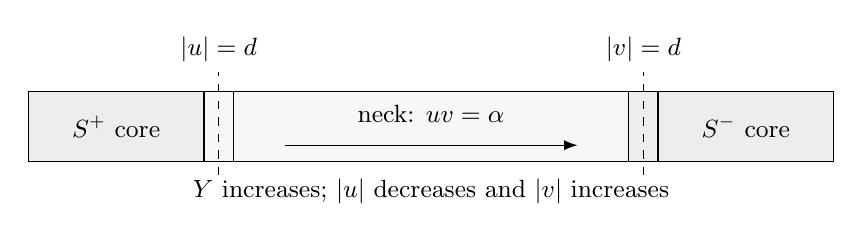
\begin{tikzpicture}[x=0.93cm,y=0.85cm,>=Latex,font=\small]
 \fill[black!7] (0,0) rectangle (2.8,1.05);
 \fill[black!3] (2.4,0) rectangle (8.6,1.05);
 \fill[black!7] (8.2,0) rectangle (11,1.05);
 \draw (0,0) rectangle (2.8,1.05);
 \draw (2.4,0) rectangle (8.6,1.05);
 \draw (8.2,0) rectangle (11,1.05);
 \draw[dashed] (2.6,-0.2) -- (2.6,1.35);
 \draw[dashed] (8.4,-0.2) -- (8.4,1.35);
 \node at (1.2,0.53) {$S^+$ core};
 \node at (5.5,0.72) {neck: $uv=\alpha$};
 \node at (9.8,0.53) {$S^-$ core};
 \draw[->] (3.5,0.25) -- (7.5,0.25);
 \node[above] at (2.6,1.35) {$|u|=d$};
 \node[above] at (8.4,1.35) {$|v|=d$};
 \node[below] at (5.5,-0.1) {$Y$ increases; $|u|$ decreases and $|v|$ increases};
\end{tikzpicture}
\caption{The core--neck joins in logarithmic height, not to scale.
The overlap widths are fixed.  Once $d$ is fixed, the neck length
grows as $\alpha\to0$, while its transverse width stays bounded
below.  After sewing, the same parameter $p$ labels a leaf across
both joins.}
\label{deg:neck-figure}
\end{figure}

Figure~\ref{deg:neck-figure} separates the fixed-width overlaps from
the part of the cylinder whose length grows.  Only the former
enter the local transition estimates.

\begin{lemma}[Buffered seams]\label{deg:seams}
There are fixed positive parameter and seam widths and a fixed
bound on translation derivatives with the following property.
Choose $d$ sufficiently small, then $\alpha\neq0$ sufficiently
small depending on $d$.  At matching nominal end positions the
normalized core and neck charts have degree-one symplectic
transitions of the form
\[
         F_j=J_j\circ(\operatorname{id}+E_j),\qquad
         J_j(w,p)=(w+a_j(p),p),
\]
on buffered seams.  After choosing long-coordinate origins and
cut heights, they satisfy the domain hypotheses of
Theorem~\ref{sew:chain}, apart from exactness, and
\[
                     \sup_j\|E_j\|\leq C d+\epsilon(d,\alpha),
              \qquad \epsilon(d,\alpha)\longrightarrow0
                            \quad(\alpha\to0, d\text{ fixed}).
\]
The widths and the bound for $a_j'$ can be chosen before $d$.
\end{lemma}

\begin{proof}
At an exit seam Equation~\eqref{deg:exit} has leading part
$u=k_+(p)z$.  Taking a local logarithm of the nonzero coefficient
gives a change $w_{\rm neck}=w_{\rm core}+a(p)$.  Its derivative
is bounded by the logarithmic derivative of $k_+$.  Its transverse
change is exactly the identity at leading order: both parameters
are primitives of the same signed residue differential, with
the same constant at the matching nominal end.

At the entrance into the next component, the leading relation is
$v=k_-(p')/z'$ and $uv=\alpha$.  Hence $z'$ is a nonzero
holomorphic multiple of $u$, so again $w'=w+a(p)$, with the same
orientation.  The sign of the residue changes between the two
components, and the use of $z'=\infty$ at the entrance changes
it once more.  The transverse primitives therefore again agree
as germs.  The potentially large constant $\log\alpha$ affects
the translation itself, not its derivative in $p$.

The actual seam maps differ from these leading maps by $O(d)$
from the expansions and Equation~\eqref{deg:neck-normalization},
plus the core deformation error $\epsilon(d,\alpha)$.  These
estimates are in $(\log u,t)$ or $(\log v,t)$ coordinates.  The
leading changes are uniformly invertible there.  The inverse
function theorem with the reserved buffers therefore produces
the actual inverse branches throughout the seams.  Local branches
agree by uniqueness near the specified leading branch, including
after going once around the period.  Their lifts have degree one,
and they are symplectic because both charts pull back the same
surface form to $dw\wedge dp$.

For completeness, the cuts can be prepared without imposing
incompatible origins at the two ends of a block.  Work first in
raw coordinates.  Enlarge each core range to
$cd<|z|<1/(cd)$ with a fixed sufficiently small $c>0$, and add
fixed logarithmic buffers to every neck.  At a seam choose the
two matching cut heights by its leading formula at the nominal
center.  Each raw block has independent room for the choice of
its two cuts.  Then translate its single long-coordinate origin
so that its entrance is at height zero; its exit defines $L_j$.
For small $d$, and then small $\alpha$, all core and neck lengths
are at least one.  Shrink the fixed transverse discs so that
the variation of $\operatorname{Im}a_j$ about its central value
is less than $h/8$.  The logarithmic derivative bounds show that
this shrinking is independent of $d$ and $\alpha$.  The two
cut heights then give precisely
$|\operatorname{Im}a_j+L_j|<h/8$ with the required margins.
\end{proof}

\subsection{Infinite continuation and transverse partners}

We spell out the compactness statement needed for an infinite
construction.  The finite atlas has larger and smaller end-position
patches whose interiors cover $E$.  At a designated end choose a
regular family and a neck patch whose smaller patches contain it.
Their larger patches give a uniform positive buffer, after taking
a finite refinement if necessary.  Thus a transverse translation
whose size is less than a fixed threshold still belongs to the
chosen larger patches, for every designated position on $E$.
Both orderings of the ends of a core are included in the atlas.
If a later choice requires a smaller positive working radius,
use more centers from these same compact families.  Their smaller
end-position neighborhoods again cover $E$, and a finite subcover
can be chosen.  These are restrictions and translations of the
same raw charts, so the uniform derivative and buffer bounds do
not change.  In particular, the positive parameter width retained
by the sewing theorem can be fixed before the cutoff $d$ without
losing coverage.

Start with any prescribed core or neck chart.  Match its outgoing
nominal end with a new chart.  By Lemma~\ref{deg:seams} its period
defect is $O(d+\epsilon(d,\alpha))$.  Apply
Lemma~\ref{sew:centers} to make the seam exact, translating the
actual and model transverse coordinates of the newly added chart
together.  Use that updated model's outgoing end for the next
choice.  It is some point of $E$, where another uniformly
buffered choice is available.  Continue alternately through
cores on the two components and intervening necks.  In the
opposite direction perform the corresponding adjustment on
each newly added input block.  The initial block need not be
moved in either construction.

The displacement of the nominal centers over many steps can be
large.  This causes no loss of the estimates: at each step the
comparison is with that block's own translated model on a
larger prepared patch, and the outgoing model position is
updated before the following seam is formed.  The set of
possible positions is the whole compact curve $E$, not a
single fixed local parameter disc.  The actual parameter disc
in each centered chart, in contrast, has the same fixed radius.
This is exactly the distinction used in
Lemma~\ref{sew:centers}.

Take $d$ small and then $\alpha$ small enough that all seam
errors, including the period adjustments, are below the threshold
of Theorem~\ref{sew:chain}.  We obtain periodic symplectic
immersions of $\C\times\Delta_b$ whose corrected charts are
uniformly close to the corresponding raw charts.  By making the
initial errors smaller, their first derivatives on the fixed
interior core patches are as close as required.

At a designated interior crossing use an additional chain starting
from the transverse partner pencil.  In the central model the
two tangent directions have a fixed positive angle in the chosen
local coordinates.  The two corrected families still have
independent directions there, and the partner chart still covers
a smaller neighborhood of the crossing.  For every sufficiently
small transverse parameter on the first strip, a point on its
leaf in this core patch therefore lies on a leaf of the partner
family, with transverse intersection.  This uses the partner
\emph{family}: no interpolation at a prescribed point is needed.

By Remark~\ref{loc:alignment} and Proposition~\ref{loc:criterion},
these strips imply property $L$ at every covered point on the
first strip, including points in other blocks of its chain.
The unbounded coordinate may be translated to the crossing,
and the common parameter $p$ identifies the same leaf all along
the chain.  A strip initialized in a neck reaches one of the
adjacent prescribed regular core families and uses its chosen
partner in exactly this fashion.

\subsection{Coverage and unrestricted deformation}

There are two coverage issues: the middle of an increasingly long
neck and the neighborhood of either cutoff.  Neither may be
discarded as a small set.  We verify them in coordinates with
uniform bounds.

Inside a core away from its ends, the deformed chart and its
sewing correction are close in $C^1$ to the central regular
chart.  Local invertibility with a margin implies that its image
contains every prescribed smaller regular patch, under a local
identification of the smooth fibers.  This includes the compact
boundary patches of all the coordinate discs chosen earlier.
The same statement is uniform over compact subfamilies and
small recenterings.

For a neck, the normalized raw map is already a coordinate chart
in $(\log u,t)$ on the whole buffered interval from $|u|\asymp d$
to $|v|\asymp d$.  The correction supplied by
Theorem~\ref{sew:chain} is uniformly close to the identity in
$(w,p)$ and is defined with fixed margins, independently of
the interval length.  Its image contains a uniformly smaller
source cylinder: at any point of that smaller cylinder, a
fixed-radius coordinate ball lies in the larger one, and the
small-change inverse theorem applies there.  Thus the corrected
chart covers the entire smaller neck interval and the smaller
end-position patch, not only a compact part chosen in advance.

At the $u$-cut use a normal-crossing patch about a point of $E$.
On the component side, Equations~\eqref{deg:entrance} and
\eqref{deg:exit} give uniformly nonsingular leading coordinates
$(\log u,t)$, with error $O(|u|)$.  The coordinate $t$ differs
from the endpoint coordinate by $O(|u|)$.  Choose a fixed small
normal size $d_*>0$, smaller than a fixed fraction of the
available end-position width.  The selected core charts cover
the region from a fixed multiple of $d$ up to $d_*$, after
shrinking their end-position patches.  Their sewing corrections
are uniformly small in the same logarithmic coordinates.
The neck chart covers below that multiple of $d$ and overlaps
the core region by its extra logarithmic buffers.  The identical
argument applies at the $v$-cut.  A finite collection of the
smaller end-position patches covers $E$.

This argument does not ask for a lower bound on an ordinary
metric chart radius at $|u|=d$.  All inverse estimates there
are in logarithmic and end-position coordinates, where the
leading maps and the buffers have uniform bounds.  One first
chooses the position widths and the needed error bound for
coverage and for the core crossings, and then chooses $d$.
The fixed $d_*$ can be reduced after the widths are chosen;
finally take $d$ much smaller than $d_*$.  On the remaining
compact region outside these end neighborhoods, the preceding
finite collection of regular patches and coordinate discs
applies.  If the end neighborhoods have been reduced in choosing
$d_*$, the intervening closed annular region is already covered
by the same regular core families; it is a fixed compact region
before $d$ is chosen.  Properness of the semistable family ensures that
these core and neck regions cover every nearby smooth fiber.

At each reserved coordinate disc away from $E$, use the
submersion coordinates of the total space to transport its
local coordinate construction to the smooth fibers.  Its
boundary, and the boundaries of sufficiently nearby translated
or tilted discs, remain in the regular patches where $L$ was
just proved.  Corollary~\ref{loc:disc} gives $L$ throughout the
remaining smaller coordinate neighborhoods.  Thus $L$ holds
at every point of the selected smooth quartic.

Now fix the small nonzero $\alpha$ used above.  Every raw core
and neck chart is a map from a \emph{finite} annulus times a
disc, with margins.  There are finitely many raw charts;
all the moving versions are restrictions and translations of
these larger charts.  Apply Lemma~\ref{loc:deformation} in the
full local deformation family of this smooth K3, choosing a
nearby holomorphic symplectic form and normalizing each chart.
They deform simultaneously with arbitrarily small additional
error.  Their seam inverse branches persist: on each compact
buffered seam they are the nearby branches of the original
local inverse, and uniqueness makes those branches agree
throughout the seam and around its period circle.  Thus all
the domain, derivative, period-adjustment, coverage, and
transversality estimates persist in a sufficiently small
unrestricted deformation neighborhood.  This argument does
not deform the infinitely many corrected charts individually;
it deforms the finite raw atlas and repeats its uniformly
controlled construction.

The order of choices is worth recording because it prevents
any dependence of the allowable error on the length of the
neck:
\begin{enumerate}
 \item Choose the finite compact regular families, partner
       crossings, end-position patches, disc boundaries,
       parameter widths and logarithmic buffers.
 \item Choose an allowable sewing and coverage error for
       these data; the derivative bounds in the leading
       shears have already been fixed.
 \item Choose $d$ so that the $O(d)$ errors are below that
       allowance, and then choose a nonzero $\alpha$ so that
       all fixed-$d$ deformation errors are below it.
 \item Choose the full deformation neighborhood of that
       fixed smooth quartic so that its additional errors
       remain within the same allowance.
\end{enumerate}

K3 deformation theory gives a smooth local deformation space,
and the marked period map is a local isomorphism by local
Torelli; see \cite{Huybrechts}.  Its image of this last
neighborhood is a nonempty open subset of the full period
domain.  Any other marked K3 with the same period has an
isomorphic underlying surface: signs and reflections in
algebraic roots match the K\"ahler chambers while fixing the
period, and global Torelli then applies \cite{Huybrechts}.
Consequently every surface with a period in this open subset
has $L$ everywhere, proving
Proposition~\ref{deg:open}.  Theorem~\ref{ana:cap} consequently
gives convex approximation for each of these surfaces.

\section{Periods containing a rational direction}
\label{rat:section}

Let
\[
 \Lambda=3U\oplus 2E_8(-1),\qquad
 \mathcal D=\{P\subset\Lambda\otimes\R:
       P\text{ is an oriented positive two-plane}\}.
\]
Here positivity refers to the intersection form, denoted by $(\ ,\ )$.
For a primitive vector $v\in\Lambda$ with $(v,v)>0$, set
\[
 \mathcal D_v=\{P\in\mathcal D:v\in P\}.
\]
All open subsets of $\mathcal D_v$ below have its relative real topology.
We use the K3 period, Torelli, and lattice theorems in their usual
unpolarized form; a reference for these results and the facts about
genus-one pencils used below is
\cite[Chapters~2, 6--8, and~11]{Huybrechts}.

\begin{theorem}\label{rat:open}
For every primitive positive integral vector $v\in\Lambda$, there is a
nonempty relatively open subset $\mathcal O_v\subset\mathcal D_v$ such
that every marked K3 surface with period in $\mathcal O_v$ has property
$L$ at every point.
\end{theorem}

On a marked K3 surface whose period contains $v$, the holomorphic
symplectic form has a unique normalization satisfying
\begin{equation}\label{rat:normalization}
 [\operatorname{Im}\sigma]=v.
\end{equation}
Indeed the real and imaginary parts of a nonzero holomorphic two-form
are orthogonal and of equal positive square, and multiplication by a
nonzero complex scalar gives all oriented orthogonal frames of its
period plane. This normalization varies smoothly on $\mathcal D_v$.

We first produce a convenient central surface, then construct strips
on its nearby deformations satisfying \eqref{rat:normalization}.

\subsection{An isotrivial center for every positive integral vector}

\begin{lemma}\label{rat:center}
For every primitive $v\in\Lambda$ of square $2d>0$, there is a marked
projective K3 surface $X_0$ whose period contains $v$ and which admits
a genus-one fibration
\[
 \pi:X_0\longrightarrow\mathbb P^1
\]
with all smooth fibers of $j$-invariant zero. Its primitive fiber class
$e\in\Lambda$ satisfies $(e,v)=0$.
\end{lemma}

\begin{proof}
We begin with an auxiliary elliptic K3 surface with section, given by
the Weierstrass equation
\[
 y^2=x^3+a(t),
\]
where $a$ is a section of $\mathcal O_{\mathbb P^1}(12)$ with twelve
simple zeros, and the fundamental line bundle is
$\mathcal O_{\mathbb P^1}(2)$. The canonical bundle formula gives
trivial canonical bundle, and
$R^1\pi_*\mathcal O=\mathcal O_{\mathbb P^1}(-2)$ gives irregularity
zero. The simple zeros give cuspidal fibers with smooth total space.
Thus the smooth Weierstrass surface is a K3 surface. These global
Weierstrass and direct-image formulas are recalled in
\cite[Chapter~11, Sections~1--2]{Huybrechts}.

Let $g$ be the automorphism which multiplies $x$ by a primitive cube
root of unity. Its fixed locus is the disjoint union of the zero
section and the double cover $x=0$ of the base. The latter is branched
at twelve points and has genus five. The fixed locus has Euler
characteristic $2+(2-10)=-6$. The topological Lefschetz formula, in the order-three K3 formulation
of \cite[proof of Theorem~2.2]{ArtebaniSarti}, gives
\[
 \operatorname{tr}(g\mid H^2)=-8.
\]
If $r$ is the invariant rank, the other eigenvalues occur in conjugate
pairs of primitive cube roots, so
$r-(22-r)/2=-8$, whence $r=2$. The fiber and zero section generate a
unimodular hyperbolic plane in this invariant lattice; consequently
the invariant lattice is exactly $U$. Its orthogonal complement is
even unimodular of signature $(2,18)$ and contains two hyperbolic
planes.

That complement contains a primitive vector of square $2d$.
Eichler's criterion, applied to the unimodular K3 lattice with its
two hyperbolic summands, says that primitive vectors with the same
square are isometric \cite{Eichler}. We may therefore transport the
preceding lattice isometry so that the specified vector $v$ belongs
to its noninvariant complement. There
$1+g+g^2=0$, and thus
\[
 (v,v)=(gv,gv)=2d,\qquad (v,gv)=-d.
\]
The plane $P_0=\operatorname{span}_{\R}\{v,gv\}$ is positive. Choose
either of its two orientations, and realize it as a marked K3 period
by period surjectivity. The invariant $U$ is algebraic at this period
and contains a positive integral class, so the resulting surface is
projective.

Choose a primitive isotropic generator $e$ of this $U$, with sign
chosen so that its represented class is effective. We keep the abstract
lattice data $g,U,e$ fixed and change the marking by reflections in
algebraic $(-2)$-classes so that the class represented by $e$ becomes
nef. The reflections fix $P_0$ pointwise, hence fix $v$; all preceding
lattice relations are unchanged.
For completeness, if an effective isotropic class has negative
intersection with an irreducible curve, that curve is a $(-2)$-curve;
reflection in it reduces the positive integral degree against a
fixed ample class. Repetition terminates in the nef cone. The
primitive nef isotropic pencil theorem then gives a base-point-free
complete pencil $|e|$ with
\[
 h^0(\mathcal O(e))=2,\qquad H^1(\mathcal O(e))=0.
\]
It defines a genus-one fibration on our center.

We must show that this particular pencil is isotrivial. The
$g$-invariant period planes of the chosen eigenvalue form a complex
ball: they are the positive lines in one of the two nonreal
eigenspaces of $g$ on $U^\perp\otimes\C$. Take a small ball through
$P_0$, realized by a marked local K3 family. At a generic point its
algebraic lattice is precisely $U$. To see this, each integral class
outside $U$ imposes a proper linear Hodge condition; such a condition
cannot vanish on the entire eigenspace because the two conjugate
eigenspaces span $U^\perp\otimes\C$. Their countable union has empty
interior.

The line bundle with class $e$ extends to this small family. One way
to verify the extension is to take a contractible Stein base. The
topological class extends to the total space and has zero image in
$H^2(\mathcal O)$: by the Leray spectral sequence and Stein
vanishing this group is the space of sections of
$R^2\pi_*\mathcal O$, and the class vanishes fiberwise because it is
of type $(1,1)$. The exponential sequence supplies the line bundle.
The vanishing of $H^1(\mathcal O(e))$ and cohomology and base change
extend its two sections. Their having no common zero is open by
properness. Thus the genus-one pencils persist near $P_0$.

At every nearby generic period, $g$ acts identically on the Picard
lattice, hence fixes an ample class. Global Torelli realizes it as
an automorphism of order three. Suppose its induced action on the
pencil base were nontrivial. All its fixed points would then lie
over the two fixed points of that base action. Every fixed curve
would be vertical. Since an irreducible vertical curve $C$ satisfies
$(C,e)=0$, the Hodge index theorem gives $C^2\leq0$ and adjunction
gives $p_a(C)\leq1$. The fixed locus of a finite-order automorphism
of a smooth surface is a disjoint union of smooth curves and
isolated points. It would therefore have nonnegative Euler
characteristic, contrary to the value $-6$ determined by the
cohomological action.

The base action is consequently trivial. The multiplier on a
smooth fiber's holomorphic differential equals the primitive
cube-root multiplier on the surface form. A smooth elliptic curve
with such an automorphism has $j=0$. Finally fix any smooth member
of the central pencil. It remains smooth in the extended pencil
over a neighborhood in the deformation base, and its $j$-invariant
varies continuously there. The nearby generic values are zero, so
the central value is zero as well. This proves the assertion for
every smooth member at $P_0$. The relation $(e,v)=0$ holds because
$e$ belongs to the original invariant lattice.
\end{proof}

\subsection{Actions on the smooth fibers}

Fix the surface of Lemma~\ref{rat:center} and the normalized form
$\sigma_0$. Write $S\subset\mathbb P^1$ for the finite set of
singular values. The linear monodromy of a constant-modulus family
of elliptic curves is finite. Choose a connected finite cover of
$\mathbb P^1\setminus S$ on which that monodromy is trivial, and
compactify it to a smooth compact curve $B$. Denote the resulting
punctured curve by $B^\circ$. A fixed oriented basis
$\gamma_1,\gamma_2$ now identifies the homology of all smooth
fibers over $B^\circ$.

The base change need not possess a global section. Locally it has
holomorphic sections and product torus charts. For any primitive
cycle $\gamma$ there are cylinder coordinates, with the chosen
cycle represented by the period $1$, in which
\begin{equation}\label{rat:cylinder-form}
 \sigma_0=dw\wedge dp,\qquad dp=\eta_\gamma.
\end{equation}
Here $\eta_\gamma$ is a nowhere-zero holomorphic one-form on the
corresponding base patch. Indeed, in a local product chart the
coefficient of the surface form is constant along each compact
elliptic fiber. The period normalization makes these base forms
agree on overlaps. They therefore define a global one-form
$\eta_\gamma$ on $B^\circ$. For the two basis cycles the forms
are in a constant nonreal ratio.

If $l$ is an oriented smooth loop in a K3 surface with normalized
form $\sigma$, define its action by
\begin{equation}\label{rat:action}
 H_\sigma(l)=\int_C\operatorname{Im}\sigma\pmod{\Z},
 \qquad \partial C=l.
\end{equation}
The chain $C$ exists because $H_1(X,\Z)=0$, and the value is
independent of $C$ because $[\operatorname{Im}\sigma]=v$ is
integral. On $X_0$, representatives of a fixed homology class in a
smooth elliptic fiber give the same action, since the restriction
of $\sigma_0$ to that fiber is zero. Let
\[
 h_\gamma:B^\circ\longrightarrow\R/\Z
\]
be this action function. Orientations in
\eqref{rat:cylinder-form} may be chosen so that
$dh_\gamma=\operatorname{Im}\eta_\gamma$; changing all these signs
would make no difference below. Actions are additive in the cycle.

\begin{lemma}\label{rat:safe}
The forms $\eta_\gamma$ and functions $h_\gamma$ extend to $B$.
The map
\[
 h=(h_{\gamma_1},h_{\gamma_2}):B\longrightarrow(\R/\Z)^2
\]
has finite fibers. For each primitive $\gamma$, put
\[
 F_\gamma=h_\gamma(B\setminus B^\circ).
\]
Outside a finite subset of $B$, at least two of the three cycles
$\gamma_1,\gamma_2,\gamma_1+\gamma_2$ have action outside their
respective finite sets $F_\gamma$. Any two of these cycles form an
integral homology basis.
\end{lemma}

\begin{proof}
Integration over the elliptic fibers in local product charts
expresses the pullback symplectic volume as a fixed positive
constant times $i\eta_\gamma\wedge\overline{\eta_\gamma}$.
The base change has finite degree and $X_0$ is compact, so this
one-form has finite $L^2$ norm on $B^\circ$. In a punctured local
coordinate, a holomorphic one-form with finite $L^2$ norm has no
negative Laurent coefficients. It thus extends holomorphically
across each puncture. A local primitive of the extended form
also extends the circle-valued action function.

The holomorphic forms $\eta_{\gamma_1}$ and
$\eta_{\gamma_2}$ have constant nonreal ratio. Consequently an
invertible real linear map identifies the pair of their imaginary
parts with a complex-linear differential. Endow $(\R/\Z)^2$ with this
constant complex structure. Then $h$ is a nonconstant holomorphic
map from the compact Riemann surface $B$ to an elliptic curve.
It has finite fibers.

A point without two safe choices satisfies two forbidden-level
conditions. Each pair of the integral linear functions
$h_{\gamma_1},h_{\gamma_2},h_{\gamma_1}+h_{\gamma_2}$ is an
automorphism of the real two-torus. Thus any two such conditions
restrict $h$ to a finite set of torus values. The inverse image is
finite by the preceding paragraph.
\end{proof}

We call a cycle safe at a point if its action avoids $F_\gamma$.
Every closed set of safe action values has compact inverse image
in $B^\circ$. This elementary compactness statement, rather than
a bound on the number of cylinder blocks, will control all the
successive center adjustments.

\subsection{Uniform strips after deformation}

Take a marked local deformation of $X_0$, identify its underlying
smooth fibers, and restrict its parameters to $\mathcal D_v$.
Let $X_t$ and $\sigma_t$ denote the fibers and normalized forms.
The genus-one fibration is used only on $X_0$; it is not asserted
to survive on $X_t$.

\begin{lemma}\label{rat:strips}
Fix compact families of regular torus charts on $X_0$, each
equipped with a safe primitive cycle, and suppose their actions
are separated from the corresponding forbidden values by a
positive margin. Prescribe any finite number of period cells in
these initial data. For all sufficiently small $t\in\mathcal D_v$,
each datum gives a symplectic immersed strip on $X_t$, periodic in
its long coordinate with period $1$, of positive transverse width.
On the prescribed initial cells its chart is arbitrarily close in
$C^1$ to the original cylinder chart. All widths and closeness
requirements can be chosen uniformly over the given compact data.
\end{lemma}

\begin{proof}
The centers may move after each exactness correction. We therefore
prepare the compact region in which the construction will continue
before choosing the charts. Let $\rho>0$ be a common lower bound
for the distance of the specified initial actions from their
forbidden sets. For every cycle used in the initial data, put
\[
 K_\gamma=\{b\in B:
   \operatorname{dist}(h_\gamma(b),F_\gamma)\geq\rho/4\}.
\]
This set is compact in $B^\circ$. Choose finitely many
product-torus charts covering it, with larger buffered domains
still lying in $B^\circ$. All subsequent restrictions and
recentering will use this finite atlas. We shall prove that the
updated centers remain a fixed distance inside the prepared region.

In a chart for a chosen cycle, the torus has constant lattice
$\Z+\tau\Z$, where $\operatorname{Im}\tau>0$ after choosing a
positive complementary cycle. Unroll this complementary period
while retaining $w$ modulo $\Z$. We obtain finite cylinders of
any prescribed fixed length. Starting sections can be chosen at
any fiber phase, so the chart families cover all phases, not just
a particular section.

At matching nominal base positions, successive model cylinders
are identified on their overlaps by
\begin{equation}\label{rat:model-transition}
 (w,p)\longmapsto(w+a(p),p).
\end{equation}
The functions $a$ incorporate both changes of local section and
any required number of complementary periods. The latter are
constant, because the modulus is constant. On smaller members of
the finite buffered atlas, the derivatives of the remaining
translation functions have uniform bounds. Choose long block
cores containing the prescribed cells and leave several period
cells as buffers at each end. At a joint, integral complementary
translations let the two cut heights agree at the center with a
bounded adjustment inside these buffers. Both cuts of each raw
chart may be chosen independently. After translating the long
origins, these charts have the block and overlap geometry required
by Theorem~\ref{sew:chain}. Shrinking the transverse radius makes
the variations of their cut heights uniformly smaller than the
overlap margins.

Each cylinder times its transverse disc is Stein. The local
deformation argument used earlier therefore deforms these maps
on their finite buffered domains to the nearby fibers. Although
a cylinder map is usually not injective, it is an immersion, and
on each overlap its local inverse branch close to
\eqref{rat:model-transition} is unique. The branches consequently
agree around the cylinder, including its period identification.
The resulting transition is a degree-one periodic lift. The
pulled-back forms can be normalized to $dw\wedge dp$ by the
transverse integration used in Theorem~\ref{sew:chain}.
All these constructions are uniform on the finite atlas, and
their errors tend to zero with $t$.

We next compare the action of an individual deformed block with
that of its model, before any blocks have been joined. Let $b$ be
the nominal base position of a freshly centered block, and let
$l_b$ be the image of a period loop on its zero slice. Uniformly
over the prepared charts and their allowed recenterings,
\begin{equation}\label{rat:action-comparison}
 \operatorname{dist}_{\R/\Z}
    \bigl(h_\gamma(b),H_{\sigma_t}(l_b)\bigr)<\varepsilon_t,
 \qquad \varepsilon_t\longrightarrow0.
\end{equation}
To verify this, under the fixed smooth identification the real forms
$\operatorname{Im}\sigma_t-\operatorname{Im}\sigma_0$ are exact
and tend to zero smoothly. Fix a Riemannian metric on the underlying compact manifold and let
$G$ be its Hodge Green operator. For the exact two-form
$\eta_t=\operatorname{Im}\sigma_t-\operatorname{Im}\sigma_0$, put
$\beta_t=d^*G\eta_t$. Its harmonic projection vanishes and
$dG\eta_t=Gd\eta_t=0$, so Hodge decomposition gives $d\beta_t=\eta_t$.
Elliptic regularity makes $\beta_t$ tend to zero smoothly;
see \cite[Theorem~3.2 and Equation~(3.26)]{ChenLiHodge} for this
Hodge decomposition and Green-operator formulation. Integration of
these primitives around the model loops, together with the
small cylinders between nearby model and actual loops, proves
\eqref{rat:action-comparison}. The loop families are compact:
the base positions and fiber phases range over compact sets, and
the number of wraps in a block is fixed. The estimate depends on
the comparison of this block with its own model, not on any
previous choices of centers.

Starting from any chosen block, extend the chain in both
directions. At a joint initially use a chart with matching nominal
base position. Its actual symplectic transition is close to
\eqref{rat:model-transition}. Its period defect is the constant
\[
 \int_{\R/\Z}(P\,dW-p\,dw).
\]
Moving this candidate's transverse center by the appropriately
signed defect makes the period exactly zero. Retain this
translated actual chart as the next block, so the exact overlap
just obtained is preserved. Move its nominal center by the same
amount in the model $p$ coordinate; that updated position is used
only when selecting the following candidate block. The adjustment
is small, and comparison with the model of the newly centered
chart retains its original error bound. It remains to justify
that the nominal positions never approach a puncture.

For this purpose use the action \eqref{rat:action} on the actual
surface. Its value on the period loop of the zero slice is
constant within a block. It is also constant between adjacent
blocks. Indeed the primitive of $dw\wedge dp$ is $-p\,dw$;
the change of action between the image of a zero-slice loop and
the next zero-slice loop is the imaginary part, up to sign, of
the displayed period defect. The image loop winds once in the
next cylinder. Vanishing of the defect proves equality of its
action with that of the next zero slice. Denote this common
circle value by $c$.

Thus the single-block estimate \eqref{rat:action-comparison} reads
$\operatorname{dist}_{\R/\Z}(h_\gamma(b),c)<\varepsilon_t$
at every stage. We can now verify that the next center stays in
the prepared region. Require the action error and the change in
nominal action caused by a single center adjustment to be less
than $\rho/8$. For an initial block the conserved value $c$ has
distance greater than $7\rho/8$ from $F_\gamma$. Inductively,
a next nominal center may first be chosen at the preceding one;
the small adjustment keeps it inside the prepared region. The
exact action comparison then improves its distance from the
forbidden set to greater than $3\rho/4$. This restores a fixed
margin for the following step. The same argument applies
backwards. Thus the entire doubly infinite chain is available
with common transverse and overlap margins.

We have obtained exact symplectic transitions with uniformly
small errors and the block geometry required by
Theorem~\ref{sew:chain}. That theorem supplies the periodic strip
and arbitrarily small corrections on every prescribed compact
part of the initial block. Estimates on slightly larger domains
give the asserted $C^1$ closeness. The transverse width has a
uniform positive lower bound after the fixed margin losses.
\end{proof}

\subsection{Two cycles cannot give the same leaf}

\begin{lemma}\label{rat:two-periods}
In the setting of Lemma~\ref{rat:strips}, suppose two initial
strips are obtained from independent primitive cycles of one
central smooth torus. One can choose a finite required initial block
length and a positive $C^1$ error tolerance from the central torus
and its two cycles, before restricting the deformation parameter,
with the following property. For strips meeting these bounds, if
\begin{equation}\label{rat:destroy-fiber}
 ([\sigma_t],e)\ne0,
\end{equation}
then $L$ holds at every point of the smaller tube covered by both
initial strip charts.
\end{lemma}

\begin{proof}
Fix such a point $x$ and take one leaf of each strip through it,
using sheets whose preimages lie inside the buffered initial
blocks. Identify a smooth tube of the central torus with a disc
times that torus, and let $q$ be its smooth projection to the
torus. On a sufficiently large finite box in the universal plane
cover of the torus, the lifted projections of these two leaf
parametrizations are $C^1$ close to invertible affine maps.
The prescribed cylinder lengths may be chosen to include this
box and every lattice translate used below, with a fixed positive
buffer. These choices are made on the central model; the required
$C^1$ tolerance is then fixed on these finite buffered domains.
A small $C^1$ perturbation of an invertible affine map
is injective on a slightly smaller convex box, and its image
contains a further smaller box. We may therefore invert the
two projections and express the two leaf pieces as graphs over
one common convex box $Q$ in the torus cover. Choose this box to
contain a fundamental parallelogram for the two cycles and buffers
beyond every edge. The finite block lengths were chosen large
enough to accommodate these translates and buffers.

Each graph is periodic under its own primitive cycle wherever
both points and the required buffers belong to $Q$. To check
this exact assertion, shifting $w$ by $1$ leaves its strip map
unchanged. The lift of its torus projection changes by an
integral lattice vector; closeness to the original chart forces
that vector to be exactly the chosen cycle. Inversion and
uniqueness in the buffered box give the claimed graph equality.

Suppose the two holomorphic curve germs at $x$ were equal. The
set where the graph germs agree is open in $Q$. It is also
closed. At a limit of such points, both graph images have the
same limiting point. In small immersion charts at that point,
the two embedded holomorphic curve germs have accumulating
intersections, so the identity theorem makes them equal.
The use of the smooth projection causes no difficulty here:
it only supplies graph coordinates, while the identity theorem
is applied in holomorphic surface charts. Connectedness of $Q$
now makes the graphs agree throughout $Q$.

The common graph is
periodic under both edge identifications. It consequently
defines a compact smooth torus mapped into the tube whose local
image is a holomorphic curve. Let $m$ be the index of the
sublattice generated by the two cycles in the full period
lattice. Contraction of the disc component shows that the
represented integral homology class in $X_t$ is $m e$, with
$m>0$; in the application from Lemma~\ref{rat:safe}, $m=1$.
The pullback of $\sigma_t$ to a holomorphic curve is zero,
contradicting
\eqref{rat:destroy-fiber}. The two leaf germs are therefore
distinct.

They need not be transverse at $x$. Take a local foliation chart
for the second strip. Its transverse coordinate restricts to a
nonconstant holomorphic function on the first leaf, since the
two germs are distinct. Its derivative is nonzero at points
arbitrarily close to $x$. At such a point the first leaf meets
a member of the second strip family transversely. Apply
Remark~\ref{loc:alignment} at this intersection, assigning the
first strip, whose leaf contains $x$, to the role of $\sigma_2$
and the transverse partner to the role of $\sigma_1$.
Proposition~\ref{loc:criterion} then gives $L$ at $x$ by the
permitted displacement along the $\sigma_2$ leaf.
\end{proof}

\begin{proof}[Proof of Theorem~\ref{rat:open}]
By Lemma~\ref{rat:safe}, all central fibers except finitely many
have two independent safe cycle choices. Let $A\subset X_0$ be
the union of the excluded fibers and the singular fibers. This
is a proper analytic subset of dimension at most one.

We make a finite compact preparation before deforming. At every
point of $X_0\setminus A$, choose smaller regular torus patches
with two safe cycles and larger buffered patches. At a point of
$A$, choose a small holomorphic coordinate line disc through the
point whose boundary avoids $A$. Such a disc exists because a
generic line is not contained in $A$ and meets it discretely.
Two sufficiently small different tilts give transverse discs
with boundaries still outside $A$. Their centers may vary in a
smaller coordinate neighborhood. Compactness of $X_0$ permits
a finite choice of these center neighborhoods and regular
patches. Enlarge the compact regular data to include all the
disc boundaries. Every selected safe action then has a positive
common margin from its finite forbidden set.

Apply Lemma~\ref{rat:strips} to these finitely prepared data,
with blocks long enough for Lemma~\ref{rat:two-periods}.
On all sufficiently small deformations in $\mathcal D_v$, the
initial charts still cover fixed smaller tube patches, and the
coordinate-disc boundaries remain in those patches. If
\eqref{rat:destroy-fiber} holds, Lemma~\ref{rat:two-periods}
gives $L$ at every point of the required regular patches.
Corollary~\ref{loc:disc} gives $L$ in the reserved center
neighborhoods. Thus $X_t$ has $L$ everywhere.

Finally \eqref{rat:destroy-fiber} holds on a nonempty relatively
open subset arbitrarily close to $P_0$ in $\mathcal D_v$.
Indeed $(e,v)=0$, but the functional $(e,\cdot)$ does not vanish
identically on the positive vectors of $v^\perp$. Varying the
other normalized positive direction therefore breaks the
equation $(e,[\sigma_t])=0$. Local Torelli identifies our small
deformation neighborhood with a period neighborhood, giving
the desired nonempty relatively open set $\mathcal O_v$.
For any other marked K3 with the same period, global Torelli
after matching K\"ahler chambers identifies the underlying
surface, so the property has the stated period-theoretic scope.
\end{proof}

\section{Period dynamics and the conclusion}
\label{dyn:section}

We now pass from the two open regions constructed above to every
K3 surface. The distinction between no rational direction, one
rational direction, and a rational plane is essential. In
particular, density of an Oka locus alone would not justify this
step. The corrected period-orbit analysis is due to Verbitsky
\cite{VerbitskyErratum}; the recent dense-period application in
\cite{XieZhao} uses the same broad strategy of geometric flexibility, arithmetic
period dynamics, and Torelli theory. Here the two preceding geometric
constructions supply open regions for both nonrational orbit types.
We give the particular group argument needed for this transfer.

Write $V=\Lambda\otimes\R$, and let
$G=\operatorname{SO}_0(V)$ be the identity component. Passing to
finite-index subgroups, the integral isometry group gives an
arithmetic lattice $\Gamma\subset G$ by the arithmetic lattice
theorem \cite{BorelHarishChandra}.

\begin{lemma}\label{dyn:orbits}
Let $P\in\mathcal D$.
\begin{enumerate}
\item If $P\cap(\Lambda\otimes\Q)=\{0\}$, its integral-isometry
orbit is dense in $\mathcal D$.
\item If $P\cap(\Lambda\otimes\Q)=\Q v$ for a primitive integral
vector $v$, its orbit under integral isometries fixing $v$ is
dense in $\mathcal D_v$.
\end{enumerate}
\end{lemma}

\begin{proof}
We first work with an ordered orthonormal positive frame of $P$.
Its connected pointwise stabilizer is
$H=\operatorname{SO}_0(1,19)$. This group is generated by
one-parameter unipotent subgroups. Ratner's orbit closure
theorem \cite{Ratner}, applied to $H\cdot e\Gamma$ in
$G/\Gamma$, gives
\[
 \overline{H\cdot e\Gamma}=S\cdot e\Gamma
\]
for a connected closed subgroup $H\subset S\subset G$ such
that $S\cap\Gamma$ is a lattice in $S$. Thus $H$ is the
pointwise stabilizer of the actual plane $P$ throughout, and the lattice
matrices in every intermediate group are rational in the
original lattice coordinates.

Put $W=P^\perp$. As a module for
$\mathfrak h=\mathfrak{so}(W)$, the orthogonal block-matrix
decomposition is
\[
 \mathfrak{so}(V)
 =\mathfrak h\oplus\mathfrak{so}(P)\oplus(W\otimes P).
\]
The standard real representation $W$ is absolutely irreducible.
Thus an intermediate Lie algebra obtains its mixed part by
choosing a subspace $A\subset P$, with mixed module $W\otimes A$.
If $\dim A=2$, brackets give the full Lie algebra. If
$\dim A=1$, they give
$\mathfrak{so}(W\oplus A)$, the stabilizer of the positive line
$A^\perp\cap P$. Including the nonzero rotation algebra of $P$
in this case generates the missing mixed summand and hence the
full algebra. If $A=0$, the only possibilities are
$\mathfrak h$ and
$\mathfrak h\oplus\mathfrak{so}(P)$.

The proper alternatives force rational directions in $P$.
For the stabilizer of one positive line, Borel density
\cite{BorelDensity} makes its lattice Zariski dense in that
stabilizer. As the lattice consists of rational matrices, its
Zariski closure is defined over $\Q$. Its fixed line is therefore
rational. The same reasoning for $H$ makes its fixed plane
rational.

There is also no difficulty from the compact rotation factor in
the remaining algebra. Up to finite isogeny the corresponding
connected group is
$\operatorname{SO}_0(W)\times\operatorname{SO}(P)$.
Projection to the first factor is proper because its kernel is
compact. Thus the image of the lattice meets each compact set
in only finitely many points and is discrete. The finite
invariant measure on the original quotient pushes forward to
a finite invariant measure on the projected quotient, so the
image is a lattice there. Borel density implies that the
Lie algebra of the Zariski closure of the original lattice
surjects onto $\mathfrak h$. Its derived algebra is exactly
$\mathfrak h$: it is contained there because the other factor
is commutative, and it maps onto $\mathfrak h$ because that
algebra is simple. The Zariski closure and its derived algebra
are defined over $\Q$, so the fixed space of the derived
algebra, namely $P$, is rational. Here the rationality of the
Zariski closure of rational matrices follows directly from the
vanishing equations: in each bounded degree their linear
conditions have rational coefficients and hence a rational
basis of solutions.

If $P$ has no rational direction, none of these proper
alternatives is possible. Ratner's closure is consequently the
whole homogeneous space. Equivalently $H\Gamma$ is dense in
$G$. Inversion makes $\Gamma H$ dense as well, and projection
to $G/H$ makes the $\Gamma$-orbit of the chosen frame dense in
frame space.
The projection from frame space to $\mathcal D$ proves the first
assertion. The use of the frame stabilizer $H$, rather than
$H\times\operatorname{SO}(2)$, is what permits the application
of Ratner's theorem.

For the second assertion, restrict to $v^\perp$, of signature
$(2,19)$. The integral stabilizer of $v$ is arithmetic and gives
a lattice in $G_v=\operatorname{SO}_0(v^\perp)$. More explicitly,
the subgroup of integral isometries of the orthogonal lattice
acting trivially on its discriminant group extends to the full
K3 lattice while fixing $v$ \cite[Chapter~14, Section~2]{Huybrechts},
so the integral stabilizer has
finite index in the relevant orthogonal arithmetic group.

An oriented plane containing $v$ is equivalent to a positive
unit vector $u\in v^\perp$: choose the sign of $u$ using the
given plane orientation. The connected stabilizer of $u$ is
again $H=\operatorname{SO}_0(1,19)$. This time
\[
 \mathfrak{so}(2,19)=\mathfrak h\oplus W
\]
as an $\mathfrak h$-module, so irreducibility shows that $H$ is
maximal at Lie algebra level. Ratner's alternatives are a closed
$H$-orbit or a dense orbit. In the closed case Borel density
makes the line $\R u$ rational in the rational quadratic space
$v^\perp$. This would give a second rational direction in $P$,
contrary to the hypothesis. The orbit is therefore dense.
The connected group $G_v$ is transitive on positive unit
vectors, so the resulting density is throughout $\mathcal D_v$.
\end{proof}

\begin{proof}[Proof of Theorem~\ref{thm:main}]
Choose a marking of $X$ and let $P\in\mathcal D$ be its period.
The rational dimension of $P\cap(\Lambda\otimes\Q)$ is zero,
one, or two. We show in each case that $X$ has $L$ everywhere.

If it is zero, Lemma~\ref{dyn:orbits} makes the marked period
orbit dense in $\mathcal D$. It meets the nonempty open subset
provided by Proposition~\ref{deg:open}. Re-marking does not change
the complex surface. Moreover K3 surfaces with the same marked
period are isomorphic after their markings are forgotten: signs
and reflections in algebraic roots match their K\"ahler
chambers, and global Torelli then supplies an isomorphism.
Thus the all-point property $L$ in that open region holds on $X$.

If the rational dimension is one, let $v$ be a primitive
integral generator of that direction. It is positive because
$P$ is positive. The second part of Lemma~\ref{dyn:orbits}
allows us to re-mark within the stabilizer of $v$ so that the
period lies in the relatively open set $\mathcal O_v$ of
Theorem~\ref{rat:open}. The same Torelli argument gives $L$
everywhere on $X$. Notice that this step uses an open subset
inside the fixed-v locus itself.

If the rational dimension is two, $P$ is a rational plane.
Its rational orthogonal complement has signature $(1,19)$.
The positive cone is open and nonempty, so it contains a
rational vector, which can be multiplied by an integer to give
a positive integral $(1,1)$-class. The K3 projectivity criterion
implies that $X$ is projective. Proposition~\ref{prj:strips}
therefore gives $L$ at every point of $X$.

Theorem~\ref{ana:cap} now applies to $X$, proving the stated
approximation statement with all its quantifiers. The estimates
there are compact-uniform estimates for maps into $X$.
On the compact target, any two smooth Hermitian distances are
uniformly equivalent, so the conclusion holds for the
arbitrary metric specified in the statement.
\end{proof}

\section{Interpolation and further consequences}
\label{sec:dense-entire}

\subsection{Interpolation and dense immersions}

We now obtain approximation and interpolation from open Riemann
surfaces and derive the dense entire immersion in
Corollary~\ref{cor:dense}.  An \emph{open Riemann surface} is a
connected noncompact Riemann surface.  A compact subset is
\emph{Runge} if its complement has no relatively compact component.
The notation $j_a^k$ records the value and derivatives through order
$k$ in local coordinates, and $d_S$ denotes any fixed distance
inducing the topology of $S$.

\begin{corollary}\label{cor:oka1}
Let $S$ be a complex K3 surface, $R$ an open
Riemann surface, $K\subset R$ a compact Runge set, and
$A=\{a_j:j\geq1\}\subset R$ a closed discrete set of distinct points.
Let $k_j\geq1$ be integers.  For every continuous map $h:R\to S$
holomorphic near $K\cup A$ and every $\epsilon>0$, there is a
holomorphic map $f:R\to S$, homotopic to $h$, satisfying
\[
 \sup_{z\in K}d_S(f(z),h(z))<\epsilon,
 \qquad j_{a_j}^{k_j}f=j_{a_j}^{k_j}h\quad(j\geq1).
\]
Finite or empty interpolation sets are also allowed.  If each
prescribed first derivative is nonzero, $f$ can be chosen to be an
immersion.
\end{corollary}

\begin{proof}
Theorem~\ref{thm:main} and the convex approximation characterization
\cite[Theorem~0.1]{ForstnericCAP} imply that $S$ is Oka.  Every Oka manifold is
Oka-1, which is precisely the approximation and interpolation
property stated here. The CAP-to-interpolation implication is
established in \cite[Corollary~1.3]{ForstnericInterpolation}; for the
Oka-1 formulation with individually prescribed jet orders, see \cite[Definition~1.1 and the following
discussion]{AlarconForstneric}.  Since $\dim_{\C}S=2$, the same
interpolating map can be chosen to be an immersion by
\cite[Corollary~2.10]{AlarconForstneric} when all prescribed first
derivatives are nonzero.
\end{proof}

\begin{proof}[Proof of Corollary~\ref{cor:dense}]
Choose a countable dense sequence $(x_j)_{j\geq1}$ in the ordinary
topology of $S$, set $x_0=x$, and choose nonzero vectors
$v_j\in T_{x_j}S$, with $v_0=v$.  At the distinct source points
$a_j=3j$, choose holomorphic germs $g_j:(\C,a_j)\to(S,x_j)$
with $g'_j(a_j)=v_j$.  Explicitly, if $\kappa_j$ is a chart taking
$x_j$ to the origin in a ball in $\C^2$, put
\[
 g_j(z)=\kappa_j^{-1}\bigl((z-a_j)d\kappa_j(v_j)\bigr).
\]
Choose $0<r_j<1/3$ so that this formula is defined near
$\{|z-a_j|\leq3r_j\}$.  These closed discs are disjoint and
locally finite.

The germs are restrictions of a single continuous map $h:\C\to S$.
To construct it, fix $b\in S$ and a continuous path from each
$x_j$ to $b$.  Use $g_j$ on $|z-a_j|\leq r_j$.  On the annulus
$r_j\leq|z-a_j|\leq2r_j$, multiply $\kappa_j(g_j(z))$ by a
continuous radial cutoff equal to one near its inner boundary and
zero near its outer boundary.  Convexity of the coordinate ball
keeps the resulting map in the chart.  On
$2r_j\leq|z-a_j|\leq3r_j$, follow the chosen path from $x_j$
to $b$ with a radial parameter constant near the two boundaries.
Put $h=b$ elsewhere.  Local finiteness and the boundary agreements
prove continuity; $h$ is holomorphic near every $a_j$ and near the
compact Runge disc $K=\{|z|\leq r_0/2\}$.

Apply Corollary~\ref{cor:oka1} to $h$, $K$,
and the closed discrete sequence $(a_j)_{j\geq0}$, prescribing the
first jet at every $a_j$.  Since every $v_j$ is nonzero, this gives
an interpolating holomorphic immersion $f:\C\to S$.  Thus
\[
 f(a_j)=x_j,\qquad f'(a_j)=v_j\quad(j\geq0).
\]
The case $j=0$ gives the prescribed point and exact tangent vector.
The image contains the dense sequence $(x_j)_{j\geq1}$, proving
ordinary density. If $S$ is projective, its Zariski closed subsets are
closed in the ordinary complex topology, proving the last assertion in
that case.
\end{proof}

\paragraph{Strong dominability.}
For every complex K3 surface $S$ and every $x\in S$, there is a
holomorphic map $F_x:\C^2\to S$ with $F_x(0)=x$ and
$d(F_x)_0:\C^2\to T_xS$ an isomorphism. This is strong dominability
by $\C^2$ in the sense of
\cite[Definition~1]{ForstnericLarussonSurfaces}.
Indeed, choose a local coordinate inverse at $0\in\C^2$ taking $0$ to
$x$, and extend it continuously to $\C^2$ by a radial cutoff inside
the coordinate ball, keeping it unchanged near $0$. The Oka property
with first-order jet interpolation at $\{0\}$
\cite[Proposition~1.2 and Corollary~1.3]{ForstnericInterpolation}
gives an entire map with the same value and differential at $0$.

\subsection{Surface classification and global sprays}
\label{sec:surface-consequences}

The K3 theorem also settles the Oka property for Enriques surfaces.
Xie and Zhao proved it for unnodal Enriques surfaces, namely those
containing no $(-2)$-curves \cite[Theorem~C and Corollary~3.5]{XieZhao}.
The following consequence includes the nodal case. Its class-VII
assertion has a separate input: the global spherical shell theorem
\cite[Theorem~1.1]{OpenAIGSS}, which is not used in the K3 proof.

\begin{corollary}[Oka surfaces in Kodaira dimension zero and class VII]
\label{cor:surface-classification}
Every complex Enriques surface is Oka. More generally, every connected
minimal compact complex surface of Kodaira dimension zero is Oka.
A connected minimal compact complex surface of class~VII is Oka if and
only if it is a Hopf surface or an Enoki surface.
\end{corollary}

\begin{proof}
Every complex Enriques surface has an unramified holomorphic K3 double cover
\cite[Introduction]{GallegoGonzalezPurnaprajna}. Its covering surface
is Oka by Theorem~\ref{thm:main}, and the Oka property descends through
holomorphic covering maps \cite[Introduction]{ForstnericLarussonSurfaces}.
This proves the Enriques assertion. Apart from K3 and Enriques surfaces,
the minimal compact complex surfaces of Kodaira dimension zero are
complex tori, bielliptic surfaces, and Kodaira surfaces, which are Oka
by the established cases recalled in
\cite[Introduction]{ForstnericLarussonSurfaces}.

A minimal class-VII surface has $b_1=1$ and $\kappa=-\infty$. When
$b_2>0$, the global spherical shell theorem
\cite[Theorem~1.1]{OpenAIGSS} therefore applies, so the surface is a
Kato surface. The class-VII decomposition recalled in
\cite[Introduction]{ForstnericLarussonSurfaces} now makes the list
exhaustive: Hopf and Inoue surfaces for $b_2=0$, and Enoki,
Inoue--Hirzebruch, and intermediate surfaces for $b_2>0$.
Theorem~4 of \cite{ForstnericLarussonSurfaces} shows that exactly the
Hopf and Enoki cases are Oka.
\end{proof}

The classification assertion is restricted to minimal surfaces; no
claim is made here for arbitrary blowups or for properly elliptic
surfaces.

A complex manifold $Y$ is \emph{elliptic} in Gromov's sense if it has
a global dominating holomorphic spray: a holomorphic vector bundle
$E\to Y$ and a holomorphic map $s:E\to Y$ such that $s(0_y)=y$
and the fiber differential $d(s|_{E_y})_{0_y}:E_y\to T_yY$ is
surjective for every $y\in Y$ \cite{GromovOka}.

\begin{corollary}[Global holomorphic sprays]\label{cor:global-spray}
Every projective complex K3 surface and every complex Enriques surface
is elliptic in Gromov's sense.
\end{corollary}

\begin{proof}
Projective complex K3 surfaces are Oka by Theorem~\ref{thm:main}.
Complex Enriques surfaces are projective
\cite[Section~2]{GallegoGonzalezPurnaprajna} and are Oka by
Corollary~\ref{cor:surface-classification}.
The conclusion follows from Forstneri\v c and L\'arusson's theorem
that every projective Oka manifold is elliptic
\cite[Theorem~1.1]{ForstnericLarussonElliptic}.
\end{proof}

This last implication requires projectivity; no assertion about a
global dominating spray on a nonprojective K3 surface is made here.


\bibliographystyle{plain}
\bibliography{references}
\end{document}
